%%%% Document type  %%%%
\documentclass[preprint,12pt,fleqn]{article}
\usepackage{ragged2e}

% \usepackage{nopageno} % no page numbers
\usepackage{placeins} % \FloatBarrier
\usepackage{upgreek, bm}

\usepackage[most]{tcolorbox}
\newtcolorbox[auto counter,number within=chapter]{definition}[1][]{
  enhanced,
  breakable,
  fonttitle=\scshape,
  title={Definition \thetcbcounter},
  #1
}

%%%% Document structure %%%%
%\usepackage{geometry}
\usepackage[verbose=true,letterpaper]{geometry}
\geometry{
    textheight=9in,
    textwidth=6in,
    top=1in,
    headheight=12pt,
    headsep=25pt,
    footskip=30pt,
}

\usepackage{lineno} % used along with \linenumbers after begin document. 
\usepackage{setspace} 
% \setstretch{1.4}
\makeatletter % The following lines get rid of footer stating pre-preint to elsevier.
\def\ps@pprintTitle{%
\let\@oddhead\@empty
\let\@evenhead\@empty
\def\@oddfoot{}%
\let\@evenfoot\@oddfoot}
\makeatother
\graphicspath{ {../images/} }
\usepackage{pgf} % calculate cohort stats percentage

%%%% Bibliography   %%%%
\usepackage{natbib}
\setcitestyle{numbers,sort&compress}
\setcitestyle{sort&compress}
\usepackage{hypernat} 
    
%%%% Aesthetics     %%%%
\usepackage{microtype}
% \RequirePackage{times} % Font
\usepackage{ccaption}
\usepackage{siunitx}
\usepackage[T1]{fontenc}
\usepackage[utf8]{inputenc}
\usepackage{nameref}% this allows a reference be named, to print unnumbered references by their section name (used here for linking to Supplemental text in this case).

%%%% Paragraph Formatting %%%
\setlength{\parindent}{0pt}
\setlength{\parskip}{6pt plus 2pt minus 1pt}

%%%% Supplemental labels%%%%
%Define command to start a supplemental section
%set the supplemental letter used for figures (e.g. Figure E1)
\newcommand{\beginsupplement}{%
        \setcounter{table}{0}
        \renewcommand{\thetable}{S\arabic{table}}%
        \setcounter{figure}{0}
        \renewcommand{\thefigure}{S\arabic{figure}}%
         }

%%%% Building tables%%%%
\usepackage{booktabs} % required for tables
\usepackage{rotating,tabularx} 
\newcolumntype{Z}{ >{\centering\arraybackslash}X } % defining table content layout per box
\usepackage{ltablex} % allow page break between lines in tabularx
% \usepackage{caption} \captionsetup{font=normalsize} % to set the caption size as normal even when table is tiny.
\usepackage{multirow}
\usepackage{pdflscape}

%%%% Colors %%%%
\usepackage{xcolor} 
\definecolor{natureblue}{RGB}{5,110,210}
    \usepackage[colorlinks]{hyperref} 
\AtBeginDocument{%this allows colours to chage from the defined elsearticle template.
\hypersetup{
    	colorlinks=true,
        linkcolor={natureblue},
    	citecolor={natureblue},
        filecolor=blue!50!black,
        urlcolor=cyan,
    	}}

\definecolor{kispiblack}{HTML}{333333}
\definecolor{kispidarkblue}{HTML}{023047}
\definecolor{kispidarkgreen}{HTML}{006666}
\definecolor{kispired}{HTML}{C70000}
\definecolor{kispilink}{HTML}{007DB8}%219EBC
% \color{kispi_black} %default
\definecolor{kispiblue}{HTML}{701A57}
% City sunset: https://www.color-hex.com/color-palette/40131
\definecolor{colorSUNSET1}{HTML}{eeaf61}
\definecolor{colorSUNSET2}{HTML}{fb9062}
\definecolor{colorSUNSET3}{HTML}{ee5d6c}
\definecolor{colorSUNSET4}{HTML}{ce4993}
\definecolor{colorSUNSET5}{HTML}{6a0d83}
\definecolor{natureblue}{RGB}{5,110,210}    
\usepackage{dirtree}  % Load the dirtree package

% command to use these colors and formatting; xspace for correct spacing including with punctuation marks.
\usepackage{xspace}
\newcommand{\variablesdarkgreen}[1]{\textbf{\textcolor{kispidarkgreen}{#1}}\xspace}
 
\usepackage{tocloft}  % Customizing the Table of Contents
\setcounter{tocdepth}{2}

%%%% Include code %%%%
% \usepackage{verbatim}
\usepackage{listings}
\lstset{
    basicstyle=\ttfamily\small,
    breaklines=true,
    postbreak=\mbox{\textcolor{red}{$\hookrightarrow$}\space}, % 
    breakatwhitespace=false,
    % frame=single,
    showstringspaces=TRUE, % Don't show spaces in strings as special characters
    tabsize=2, 
    language=sh 
}

\usepackage{fontspec}

\usepackage[printonlyused,withpage,nohyperlinks]{acronym}
\usepackage{tikz}
\usetikzlibrary{calc}
\usepackage{amsmath, amssymb}

% author affil
\usepackage{authblk}
\renewcommand\Authfont{\normalsize}
\renewcommand\Affilfont{\small}
\setlength{\affilsep}{1em}
\usepackage[printonlyused,withpage,nohyperlinks]{acronym}
\usepackage{tikz}
\usetikzlibrary{calc}
\usepackage{amsmath, amssymb}

\begin{document}
% \title{Quantifying the Genetics of Disease Inheritance for Bayesian Application}
\title{Quantifying the Genetics of Disease Inheritance in Primary Immunodeficiency}

\author[1]{Dylan Lawless\thanks{Addresses for correspondence: \href{mailto:Dylan.Lawless@kispi.uzh.ch}{Dylan.Lawless@kispi.uzh.ch}}}

\affil[1]{Department of Intensive Care and Neonatology, University Children's Hospital Zürich, University of Zürich, Switzerland.}
\maketitle
\justify

%Abstract: 150 of 150. Main text:  3931 of 4000 (intro, result, discussion, conclusion). Display (4 figures / 2 tables) of 8 total. Extended display: 13 of 10. Note that this journal uses separate online methods.


\begin{abstract}
We present an integrative framework for quantifying the prior probability of observing disease‐associated variants in any gene for a given phenotype. By combining large‐scale genomic annotation, —such as population allele frequencies and ClinVar variant classifications, with classical Hardy–Weinberg-based calculations, our method estimates observation probabilities for single nucleotide variants under autosomal dominant, autosomal recessive and X-linked inheritance. 
Applied to a panel of 557 genes implicated in primary immunodeficiency and monogenic inflammatory bowel disease, our approach generated 54,814 variant probabilities and revealed novel insights into gene constraint within functionally related pathways. 
Validation in autosomal dominant (\textit{NFKB1}) and autosomal recessive (\textit{CFTR}) disorders demonstrated close concordance between predicted and observed case counts. 
The resulting datasets, available in both machine- and human-readable formats via a Zenodo repository and a user-friendly web interface, provide robust priors to support Bayesian variant interpretation and improve clinical decision-making.
\footnote{
\noindent \textbf{Availability:} This data is integrated in public panels at 
% \url{https://switzerlandomics.ch/services/panelAppRexAi/} and 
\url{https://iei-genetics.github.io}.
The source code and data are accessible as part of the variant risk estimation project at \url{https://github.com/DylanLawless/var_risk_est}.
The variant-level data is available from the Zenodo repository:
(VarRiskEst PanelAppRex ID 398 gene variants.tsv).
VarRiskEst is available under the MIT licence.}
\end{abstract}

\noindent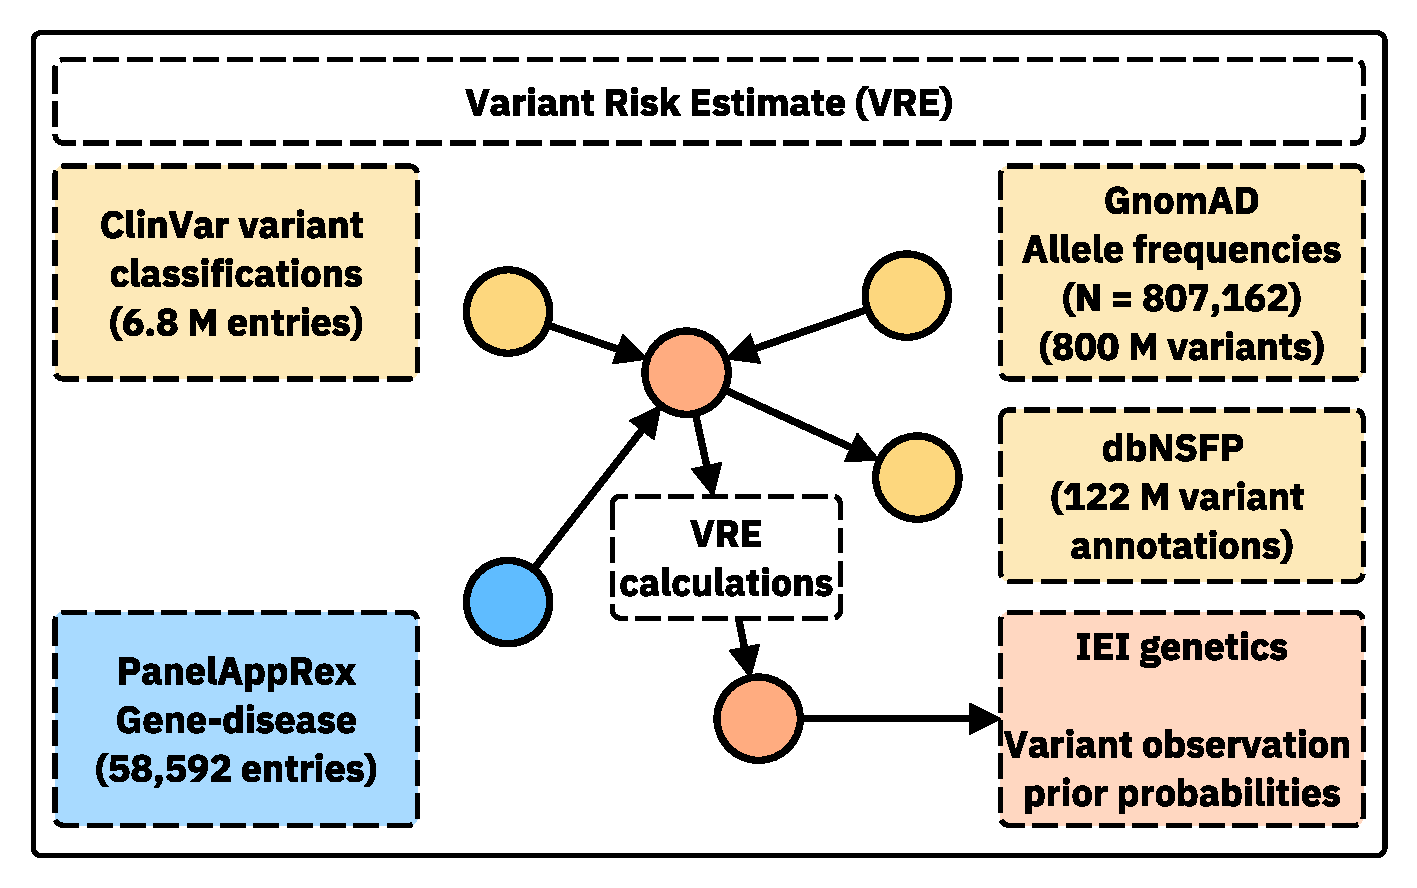
\includegraphics[width=0.99\textwidth]{../images/var_risk_est.pdf}




\clearpage

\section{Introduction}

In this study, we focused on reporting the probability of disease observation through genome-wide assessments of gene-disease combinations. Our central hypothesis was that by using highly curated annotation data - including population allele frequencies, disease phenotypes, inheritance patterns, and variant classifications - and by applying rigorous calculations based on Hardy–Weinberg equilibrium (HWE), we could accurately estimate the expected probabilities of observing disease-associated variants.

Quantifying the risk that a newborn inherits a disease-causing variant is a fundamental challenge in genomics. Classical statistical approaches grounded in HWE \cite{MayoCentury2008, AbramovsHardyWeinberg2020} have long been used to calculate genetic mode of inheritance (MOI) probabilities for single nucleotide variants (SNVs). However, applying these methods becomes more complex when accounting for different modes of inheritance, such as autosomal recessive (AR) versus autosomal dominant (AD) or X-linked (XL) disorders. In AR conditions, for example, the occurrence probability must incorporate both the homozygous state and compound heterozygosity, whereas for AD and XL disorders, a single pathogenic allele is sufficient to cause disease. 
Advances in genetic research have revealed that MOI can be even more complex \cite{zschocke_mendelian_2023}. Mechanisms such as dominant negative effects, haploinsufficiency, mosaicism, and digenic or epistatic interactions can further modulate disease risk and clinical presentation, underscoring the need for nuanced approaches in risk estimation.

We argue that our integrated approach is highly powerful because the resulting probabilities can serve as informative priors in a Bayesian framework for variant and disease probability estimation; a perspective that is often overlooked in clinical and statistical genetics. Such a framework not only refines classical HWE-based risk estimates but also has the potential to enrich clinicians’ understanding of what to expect in a patient and to enhance the analytical models employed by bioinformaticians.

PanelAppRex is a novel tool developed to aggregate disease gene panel data from multiple sources-including GE PanelApp, ClinVar, and UniProt-and to facilitate sophisticated, natural language-based searches for clinical and research applications
\cite{lawless_panelapprex_2025}. It automatically retrieves and integrates gene panels, such as those used in the NHS National Genomic Test Directory and the 100,000 Genomes Project, into machine-readable formats that support rapid variant discovery and interpretation. By enabling queries based on gene names, phenotypes, and disease groups, PanelAppRex streamlines the process of identifying disease-associated variants and enhances the efficiency of genomic diagnostics. Critical details regarding the underlying data can be found in \citet{martin_panelapp_2019, landrum_clinvar_2018, the_uniprot_consortium_uniprot_2025}.

Here, we incorporated datasets such as GnomAD, a large-scale resource that aggregates and harmonises sequencing data from diverse cohorts to provide a comprehensive view of human genetic variation \cite{karczewski2020mutational}. The v4 dataset comprises genomics data from 807,162 individuals.
Beyond its extensive catalogue of variant calls, including over 786 million single nucleotide variants and 122 million InDels, the database offers detailed annotations that support analyses of population-specific allele frequencies.

dbNSFP is a comprehensive database designed for the functional prediction and annotation of all potential non-synonymous single-nucleotide variants (nsSNVs) and splicing-site SNVs in human protein-coding genes \cite{liu_dbnsfp_2020}. It includes over 120 million variant entries and aggregates prediction scores from 33 different sources and allele frequencies from major population datasets.

ClinVar is a public archive of human genetic variation that provided detailed classifications-such as ``Pathogenic,'' ``Likely pathogenic,'' and ``Benign'' -accompanied by supporting evidence and review status \cite{landrum_clinvar_2018}. It aggregated submissions from multiple sources to present both consensus and conflicting interpretations, mapped variants to reference sequences according to HGVS standards, and collaborated with expert panels like ClinGen for ongoing re-evaluation.

We carry out validations for disease cohorts with \textit{NFKB1} 
\cite{tuijnenburgNFKB12018,
who1997primary,
cunningham1999common,
oksenhendler2008infections}
and \textit{CFTR} 
\cite{naito2023uk, castellani2013cftr2, Grasemann2023cftr}
to demonstrate autosomal dominant and recessive disease genes, respectively.

\section{Methods}
\subsection{Dataset}

Data from gnomAD v4 comprised 807,162 individuals, including 730,947 exomes and 76,215 genomes \cite{karczewski2020mutational}. This dataset provided 786,500,648 single nucleotide variants and 122,583,462 InDels, with variant type counts of 9,643,254 synonymous, 16,412,219 missense, 726,924 nonsense, 1,186,588 frameshift and 542,514 canonical splice site variants. ClinVar data were obtained from the variant summary dataset (this version: 16 March 2025) available from the NCBI FTP site, and included 6,845,091 entries, which were processed into 91,319 gene classification groups and a total of 38,983 gene classifications; for example, the gene \textit{A1BG} contained four variants classified as likely benign and 102 total entries \cite{landrum_clinvar_2018}. For our analysis phase we also used dbNSFP which consisted of a number of annotations for 121,832,908 single nucleotide variants 
\cite{liu_dbnsfp_2020}. 
The PanelAppRex core model contained 58,592 entries consisting of 52 sets of annotations, including the gene name, disease-gene panel ID, diseases-related features, confidence measurements.
\cite{lawless_panelapprex_2025}
A protein-protein interaction (PPI) network data was provided by STRINGdb, consisting of 19,566 proteins and 505,968 interactions \cite{szklarczyk2025string}.


\subsection{Variant Class Observation Probability}
As a starting point, we considered the classical Hardy–Weinberg equilibrium (HWE) for a biallelic locus:
\[
p^2 + 2pq + q^2 = 1,
\]
where \(p\) is the allele frequency, \(q = 1 - p\), \(p^2\) represents the homozygous dominant, \(2pq\) the heterozygous, and \(q^2\) the homozygous recessive genotype frequencies. For disease phenotypes, particularly under autosomal recessive (AR) inheritance, the risk is traditionally linked to the homozygous state (\(p^2\)); however, to account for compound heterozygosity across multiple variants, we extend this by incorporating the contribution from other pathogenic alleles.

Our computational pipeline estimated the probability of observing a disease-associated genotype for each variant and aggregated these probabilities by gene and ClinVar classification. This approach included all variant classifications, not limited solely to those deemed ``pathogenic'', and explicitly conditioned the classification on the given phenotype, recognising that a variant could only be considered pathogenic relative to a defined clinical context. The core calculations proceeded as follows:

\paragraph{1. Allele Frequency and Total Variant Frequency.}
For each variant \(i\) in a gene, the allele frequency was denoted as \(p_i\). For each gene, we defined the total variant frequency (summing across all reported variants in that gene) as:
\[
P_{\text{tot}} = \sum_{i \in \text{gene}} p_i.
\]
If a variant had no observed allele (\(p_i = 0\)), we assigned a minimal risk:
\[
p_i = \frac{1}{\max(AN) + 1},
\]
where \(\max(AN)\) was the maximum allele number observed for that gene. This adjustment ensured that a nonzero risk was incorporated even in the absence of observed variants.
\paragraph{2. Occurrence Probability Based on Inheritance.}
The probability that an individual was affected by a variant depended on the mode of inheritance relative to a specific phenotype. Specifically, we calculated the occurrence probability \(p_{\text{disease},i}\) for each variant as follows:
\begin{itemize}
    \item For \textbf{autosomal dominant (AD)} and \textbf{X-linked (XL)} variants, a single copy was sufficient, so
    \[
    p_{\text{disease},i} = p_i.
    \]
    \item For \textbf{autosomal recessive (AR)} variants, disease manifested when two pathogenic alleles were present. In this case, we accounted for both the homozygous state and the possibility of compound heterozygosity:
    \[
    p_{\text{disease},i} = p_i^2 + 2\,p_i\bigl(P_{\text{tot}} - p_i\bigr).
    \]
\end{itemize}

\paragraph{3. Expected Case Numbers and Case Detection Probability.}
Given a population with \(N\) births (e.g. as seen in our validation studies, \(N = 69\,433\,632\)), the expected number of cases attributable to variant \(i\) was calculated as:
\[
E_i = N \cdot p_{\text{disease},i}.
\]
The probability of detecting at least one affected individual for that variant was computed as:
\[
P(\geq 1)_i = 1 - \bigl(1 - p_{\text{disease},i}\bigr)^N.
\]

\paragraph{4. Aggregation by Gene and ClinVar Classification.}
For each gene and for each ClinVar classification (e.g. “Pathogenic”, “Likely pathogenic”, “Uncertain significance”, etc.), we aggregated the results across all variants. The total expected cases for a given group was:
\[
E_{\text{group}} = \sum_{i \in \text{group}} E_i,
\]
and the overall probability of observing at least one case within the group was calculated as:
\[
P_{\text{group}} = 1 - \prod_{i \in \text{group}} \left(1 - p_{\text{disease},i}\right).
\]

\paragraph{5. Data Processing and Implementation.}
We implemented the calculations within a high-performance computing (HPC) pipeline and provided an example for a single dominant disease gene, \textit{TNFAIP3}, in the source code to enhance reproducibility. Variant data were imported in chunks from the annotation database for all chromosomes (1--22, X, Y, M). 

For each data chunk, the relevant fields were gene name, position, allele number, allele frequency, ClinVar classification, and HGVS annotations. Missing classifications (denoted by ``.'') were replaced with zeros and allele frequencies were converted to numeric values. We then retained only the first transcript allele for simplicity, as the analysis was based on genomic coordinates. Subsequently, the variant data were merged with gene panel data from PanelAppRex to obtain the disease-related inheritance mode for each gene. For each gene, if no variant was observed for a given ClinVar classification (i.e. \(p_i = 0\)), a minimal risk was assigned as described above. Finally, we computed the occurrence probability, expected cases, and the probability of observing at least one case using the equations presented.

The final results were aggregated by gene and ClinVar classification and used to generate summary statistics that reviewed the predicted disease observation probabilities.

\subsection{Validation of Autosomal Dominant Estimates Using \textit{NFKB1}}

To validate our genome-wide probability estimates in an autosomal dominant gene, we focused on \textit{NFKB1}. Our goal was to compare the expected number of \textit{NFKB1}-related CVID cases, as predicted by our framework, with the reported case count in a well-characterised national-scale PID cohort.

\paragraph{1. Reference Dataset.}
We used a reference dataset reported by \citet{tuijnenburgNFKB12018} to build a validation model in an autosomal dominant disease gene. 
A whole‐genome sequencing study of 846 predominantly sporadic, unrelated primary immunodeficiency disease (PID) cases from the NIHR BioResource–Rare Diseases cohort  identified \textit{NFKB1} as one of the genes most strongly associated with PID. Sixteen novel heterozygous variants-including truncating, missense, and gene deletion variants-in \textit{NFKB1} were found, accounting for 46\% of common variable immunodeficiency (CVID) cases (n = 390) in the cohort. 

Functional analyses, including structural protein evaluation, immunophenotyping, immunoblotting, and ex vivo lymphocyte stimulation, revealed that all carriers exhibited deficiencies in B-lymphocyte differentiation, particularly an increased CD21low B-cell population. These findings had established heterozygous loss-of-function variants in \textit{NFKB1} as the most common monogenic cause of CVID, with significant prognostic implications.

\paragraph{2. Cohort Prevalence Calculation.}
Therefore, we used this UK-based cohort of 846 unrelated PID patients where 390 cases of CVID were attributed to \textit{NFKB1}, yielding an observed cohort prevalence of
\[
\text{Prevalence}_{\text{cohort}} = \frac{390}{846} \approx 0.461.
\]

\paragraph{3. National Estimate Based on Literature.}
Based on literature, the prevalence of CVID in the general population was estimated at approximately \(1/25\,000\)
\cite{tuijnenburgNFKB12018,
who1997primary,
cunningham1999common,
oksenhendler2008infections}.
For a UK population of \(N_{\text{UK}} \approx 69\,433\,632\), the expected number of CVID cases was calculated as
\[
E_{\text{CVID}} \approx \frac{69\,433\,632}{25\,000} \approx 2777.
\]
Thus, the maximum expected number of \textit{NFKB1}-related CVID cases in the entire population was estimated as
\[
\text{Estimated } NFKB1 \text{ cases} \approx 2777 \times 0.461 \approx 1280,
\]
with an approximate 95\% confidence interval (derived from Wilson’s method) of 1188 to 1374 cases.

\paragraph{4. Bayesian Adjustment.}
Given that the clinical cohort was derived from a specialized setting-likely capturing nearly all PID cases-the observed 390 cases may have better represented the true burden. To reconcile these perspectives, we performed a Bayesian adjustment by combining the known cohort data with the national estimate. Specifically, we computed a weighted average to symbolically acknowledge potential uncertainty:
\[
\text{Adjusted Estimate} = w \cdot 390 + (1 - w) \cdot 1280,
\]
with \(w\) set to 0.9 to reflect a strong preference for the observed data.
Additionally, we modelled the uncertainty in the observed prevalence using a beta distribution:
\[
p \sim \mathrm{Beta}(390+1,\,846-390+1),
\]
and generated 10\,000 posterior samples to obtain a density distribution for the adjusted estimate.

\paragraph{5. Validation test.}
Thus, the expected number of \textit{NFKB1}-related CVID cases derived from our genome-wide probability estimates was compared with the observed counts from the UK-based PID cohort. This comparison validated our framework for estimating disease incidence in autosomal dominant disorders.

\subsection{Validation Study for Autosomal Recessive CF Using CFTR}

To validate our framework for autosomal recessive diseases, we focused on cystic fibrosis (CF).
For comparability sizes between the validation studies, we analysed the most common single nucleotide variant (SNV) in the \textit{CFTR} gene, typically reported as ``p.Arg117His'' (GRCh38 Chr 7:117530975 G/A, MANE Select HGVSp ENST00000003084.11: p.Arg117His).
Our goal was to validate our genome-wide probability estimates by comparing the expected number of CF cases attributable to the p.Arg117His variant in \textit{CFTR} with the nationally reported case count in a well-characterised disease cohort
\cite{naito2023uk, castellani2013cftr2, Grasemann2023cftr}.

\paragraph{1. Expected Genotype Counts.}
Let \( p \) denote the allele frequency of the p.Arg117His variant and \( q \) denote the combined frequency of all other pathogenic \textit{CFTR} variants, such that
\[
q = P_{\text{tot}} - p \quad \text{with} \quad P_{\text{tot}} = \sum_{i \in \text{CFTR}} p_i.
\]
Under Hardy–Weinberg equilibrium for an autosomal recessive trait, the expected frequencies were:
\[
f_{\text{hom}} = p^2 \quad \text{(homozygous for p.Arg117His)}
\]
and
\[
f_{\text{comphet}} = 2p\,q \quad \text{(compound heterozygotes carrying p.Arg117His and another pathogenic allele)}.
\]
For a population of size \( N \) (here, \( N \approx 69\,433\,632 \)), the expected number of cases were:
\[
E_{\text{hom}} = N \cdot p^2,\quad E_{\text{comphet}} = N \cdot 2p\,q,\quad E_{\text{total}} = E_{\text{hom}} + E_{\text{comphet}}.
\]

\paragraph{2. Mortality Adjustment.}
Since CF patients experience increased mortality, we adjusted the expected genotype counts using an exponential survival model. With an annual mortality rate \(\lambda \approx 0.004\) and a median age of 22 years, the survival factor was computed as:
\[
S = \exp(-\lambda \cdot 22).
\]
Thus, the mortality-adjusted expected genotype count became:
\[
E_{\text{adj}} = E_{\text{total}} \times S.
\]

\paragraph{3. Bayesian Uncertainty Simulation.}
To incorporate uncertainty in the allele frequency \( p \), we modelled \( p \) as a beta-distributed random variable:
\[
p \sim \mathrm{Beta}(p \cdot \text{AN}_{\text{eff}} + 1,\; \text{AN}_{\text{eff}} - p \cdot \text{AN}_{\text{eff}} + 1),
\]
using a large effective allele count (\(\text{AN}_{\text{eff}}\)) for illustration. By generating 10,000 posterior samples of \( p \), we obtained a distribution of the literature-based adjusted expected counts, \(E_{\text{adj}}\).

\paragraph{4. Bayesian Mixture Adjustment.}
Since the national registry may not capture all nuances (e.g., reduced penetrance) of CFTR-related disease, we further combined the literature-based estimate with the observed national count (714 cases from the UK Cystic Fibrosis Registry 2023 Annual Data Report) using a 50:50 weighting:
\[
E_{\text{Bayes}} = 0.5 \times (\text{Observed Count}) + 0.5 \times E_{\text{adj}}.
\]

\paragraph{5. Validation test.}
Thus, the expected number of \textit{CFTR}-related CF cases derived from our genome-wide probability estimates was compared with the observed counts from the UK-based CF registry. This comparison validated our framework for estimating disease incidence in autosomal dominant disorders.

\subsection{Protein Network and Genetic Constraint Interpretation}
A protein-protein interaction (PPI) network was constructed using protein interaction data from STRINGdb \cite{szklarczyk2025string}. We previously prepared and reported 
on this dataset consisting of 19,566 proteins and 505,968 interactions 
(\url{https://github.com/DylanLawless/ProteoMCLustR}).
Node attributes were derived from log-transformed score-positive-total values, which informed both node size and colour. Top-scoring nodes (top 15 based on score) were labelled to highlight prominent interactions. To evaluate group differences in score-positive-total across major disease categories, one-way ANOVA was performed followed by Tukey HSD post hoc tests (and non-parametric Dunn’s test for confirmation). Boxplots with jittered data points were used to depict the distribution of scores by category.
GnomAD v4.1 constraint metrics data used for the PPI analysis was sourced from \citet{karczewski2020mutational}.
This provided transcript-level metrics, such as observed/expected ratios, LOEUF, pLI, and Z-scores, quantifying loss-of-function and missense intolerance, along with confidence intervals and related annotations for 211,523 observations.



\section{Results}

\subsection{Observation Probability Across Disease Genes}

Our study demonstrated that by integrating large-scale annotation databases, such as gnomAD, ClinVar, (or alternatively dbNSFP), with disease gene panels from PanelAppRex, we could systematically scan every disease-gene panel according to inheritance mode. By combining reference population allele frequencies with reported ClinVar clinical significance classifications, we calculated an expected ``observation probability'' for each single nucleotide variant (SNV). This probability represented the likelihood of encountering a variant of a given pathogenicity class for a specific phenotype.
We report the probability of disease observation for a total of 54,814 ClinVar variant classifications in 557 genes in the linked Zenodo repository (\textbf{to publish with DOI}).

In practice, our approach computed a simple observation probability for every SNV across the genome and was applicable to any disease-gene panel. Here, we focused on panels related to Primary Immunodeficiency or Monogenic Inflammatory Bowel Disease, using PanelAppRex panel ID 398 as a case study.
\textbf{Figure \ref{fig:p_varRisEst_summary_scores}} displays all reported ClinVar  variant classifications for this panel. A natural scaling system (-5 to +5) was applied to account for the frequently encountered combinations of classification labels (e.g. benign to pathogenic).
The results summarized in \textbf{Table \ref{tab:head_result_table}} illustrates that our method yielded estimations of the probability of observing a variant with a particular ClinVar classification. 
\textbf{Box \ref{box:definitions}} list the definitions for the major disease categories used throughout .
%This framework, of pre-calculated disease-related variant occurrence probabilities, enabled comprehensive analyses across the entire genome, paving the way for rapid assessment of variant significance in diverse disease contexts.

\begin{table}[ht]
\centering
\caption{Example of the first several rows from our main results for 557 genes of PanelAppRex's panel: (ID 398) Primary immunodeficiency or monogenic inflammatory bowel disease. ``ClinVar Significance'' indicates the pathogenicity classification assigned by ClinVar, while inVar Significance'' indicates the pathogenicity classification assigned by ClinVar, while ``Occurrence Prob'' represents our calculated probability of observing the corresponding variant class for a given phenotype. Additional columns, such as population allele frequency, are not shown.}
\label{tab:head_result_table} 
\centering
\resizebox{\ifdim\width>\linewidth\linewidth\else\width\fi}{!}{
\begin{tabular}[t]{lrlrllll}
\toprule
Gene & Panel ID & ClinVar Clinical Significance & GRCh38 Pos & HGVSc (VEP) & HGVSp (VEP) & Inheritance & Occurrence Probability\\
\midrule
ABI3 & 398 & Uncertain significance & 49210771 & c.47G>A & p.Arg16Gln & AR & 0.000000007\\
ABI3 & 398 & Uncertain significance & 49216678 & c.265C>T & p.Arg89Cys & AR & 0.000000005\\
ABI3 & 398 & Uncertain significance & 49217742 & c.289G>A & p.Val97Met & AR & 0.000000002\\
ABI3 & 398 & Uncertain significance & 49217781 & c.328G>A & p.Gly110Ser & AR & 0.000000002\\
ABI3 & 398 & Uncertain significance & 49217844 & c.391C>T & p.Pro131Ser & AR & 0.000000015\\
\addlinespace
ABI3 & 398 & Uncertain significance & 49220257 & c.733C>G & p.Pro245Ala & AR & 0.000000022\\
\bottomrule
\end{tabular}}
\end{table}


\begin{figure}[ht]
  \centering
  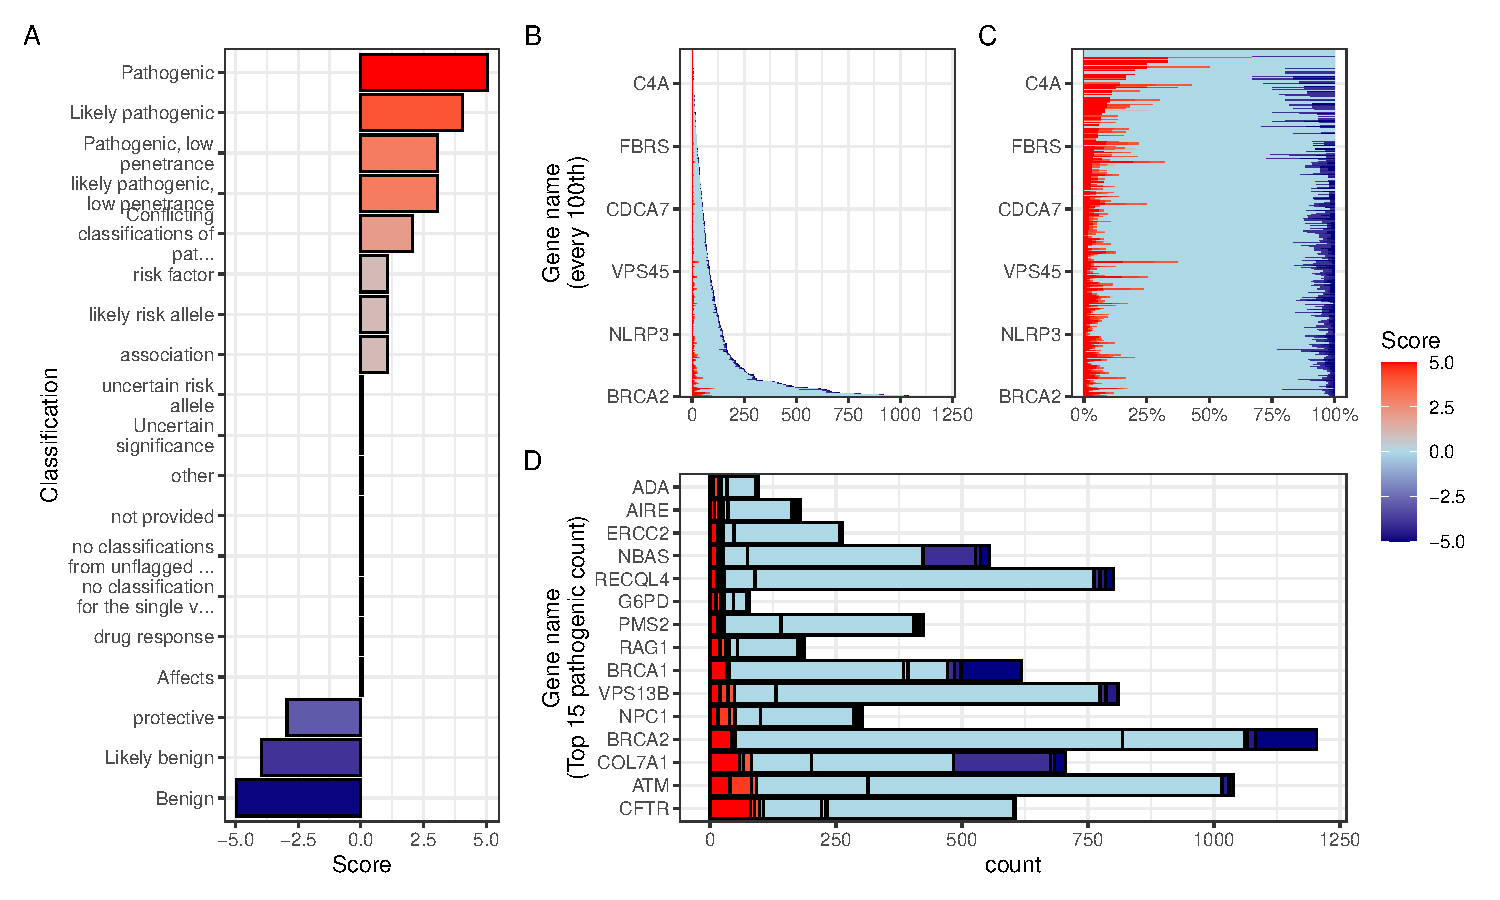
\includegraphics[width=0.99\textwidth]{../images/p_varRisEst_summary_scores.pdf}
  \caption{\textbf{Summary of ClinVar clinical significance classifications in the PID gene panel.} (A) Shows the numeric score coding for each classification. Panels (B) and (C) display the tally of classifications per gene as absolute counts and as percentages, respectively. (D) Highlights the top 15 genes with the highest number of reported pathogenic classifications (score 5).}
  \label{fig:p_varRisEst_summary_scores}
\end{figure}

\begin{tcolorbox}[colback=black!01, colframe=black!70, title=Box \ref{box:definitions} Definitions for IEI Major Disease Categories, label=box:definitions]
\textbf{Major Category} \hspace{4em} \textbf{Description}\\[5pt]
1. CID  Immunodeficiencies affecting cellular and humoral immunity\\[2pt]
2. CID+  Combined immunodeficiencies with associated or syndromic features\\[2pt]
3. PAD - Predominantly Antibody Deficiencies\\[2pt]
4. PIRD - Diseases of Immune Dysregulation\\[2pt]
5. PD - Congenital defects of phagocyte number or function\\[2pt]
6. IID - Defects in intrinsic and innate immunity\\[2pt]
7. AID - Autoinflammatory Disorders\\[2pt]
8. CD - Complement Deficiencies\\[2pt]
9. BMF - Bone marrow failure
\end{tcolorbox}



\subsection{Validation of Dominant Disease Occurrence with \textit{NFKB1}}

To validate our genome-wide probability estimates for autosomal dominant disorders, we focused on \textit{NFKB1}. We used a reference dataset from \citet{tuijnenburgNFKB12018}, in which whole‐genome sequencing of 846 PID patients identified \textit{NFKB1} as one of the genes most strongly associated with the disease, with 390 CVID cases attributed to heterozygous variants. Our goal was to compare the predicted number of \textit{NFKB1}-related CVID cases with the reported count in this well-characterised national-scale cohort.

Our model calculated 456 \textit{NFKB1}-related CVID cases in the UK. In the reference cohort,  390  \textit{NFKB1} CVID cases were reported. 
We additionally wanted to account for potential under-reporting in the reference study.
We used an extrapolated national CVID prevalence to yield an upper bound maximum of 1280 cases (95\% CI: 1188–1374), while a Bayesian-adjusted mixture estimate produced a median of 835 cases (95\% CI: 789–882). 
\textbf{Figure \ref{fig:validation_studies_bayesian_adjusted_estimates} (A)}
illustrates that our predicted value of 456 lies within these ranges and is closer to the observed count, thereby supporting the validity of our integrated probability estimation framework for autosomal dominant disorders.

\subsection{Validation of Recessive Disease Occurrence with \textit{CFTR}}

Our analysis predicted the number of cystic fibrosis (CF) cases attributable to carriage of the p.Arg117His variant (either as homozygous or as compound heterozygous with another pathogenic allele) in the UK. Based on Hardy–Weinberg calculations and mortality adjustments, we predicted approximately 648 cases arising from biallelic variants and 160 cases from homozygous variants, resulting in a total of 808 expected cases.

In contrast, the nationally reported number of CF cases was 714, as recorded in the UK Cystic Fibrosis Registry 2023 Annual Data Report
\cite{naito2023uk}. To account for factors such as reduced penetrance and the mortality-adjusted expected genotype, we derived a Bayesian-adjusted estimate via posterior simulation. Our Bayesian approach yielded a median estimate of 740 cases (95\% CI: 696, 786) and a mixture-based estimate of 727 cases (95\% CI: 705, 750).

\textbf{Figure \ref{fig:validation_studies_bayesian_adjusted_estimates} (B)} illustrates the close concordance between the predicted values, the Bayesian-adjusted estimates, and the national report supports the validity of our integrated approach for estimating disease incidence from population allele frequency data.

\begin{figure}[ht]
  \centering
  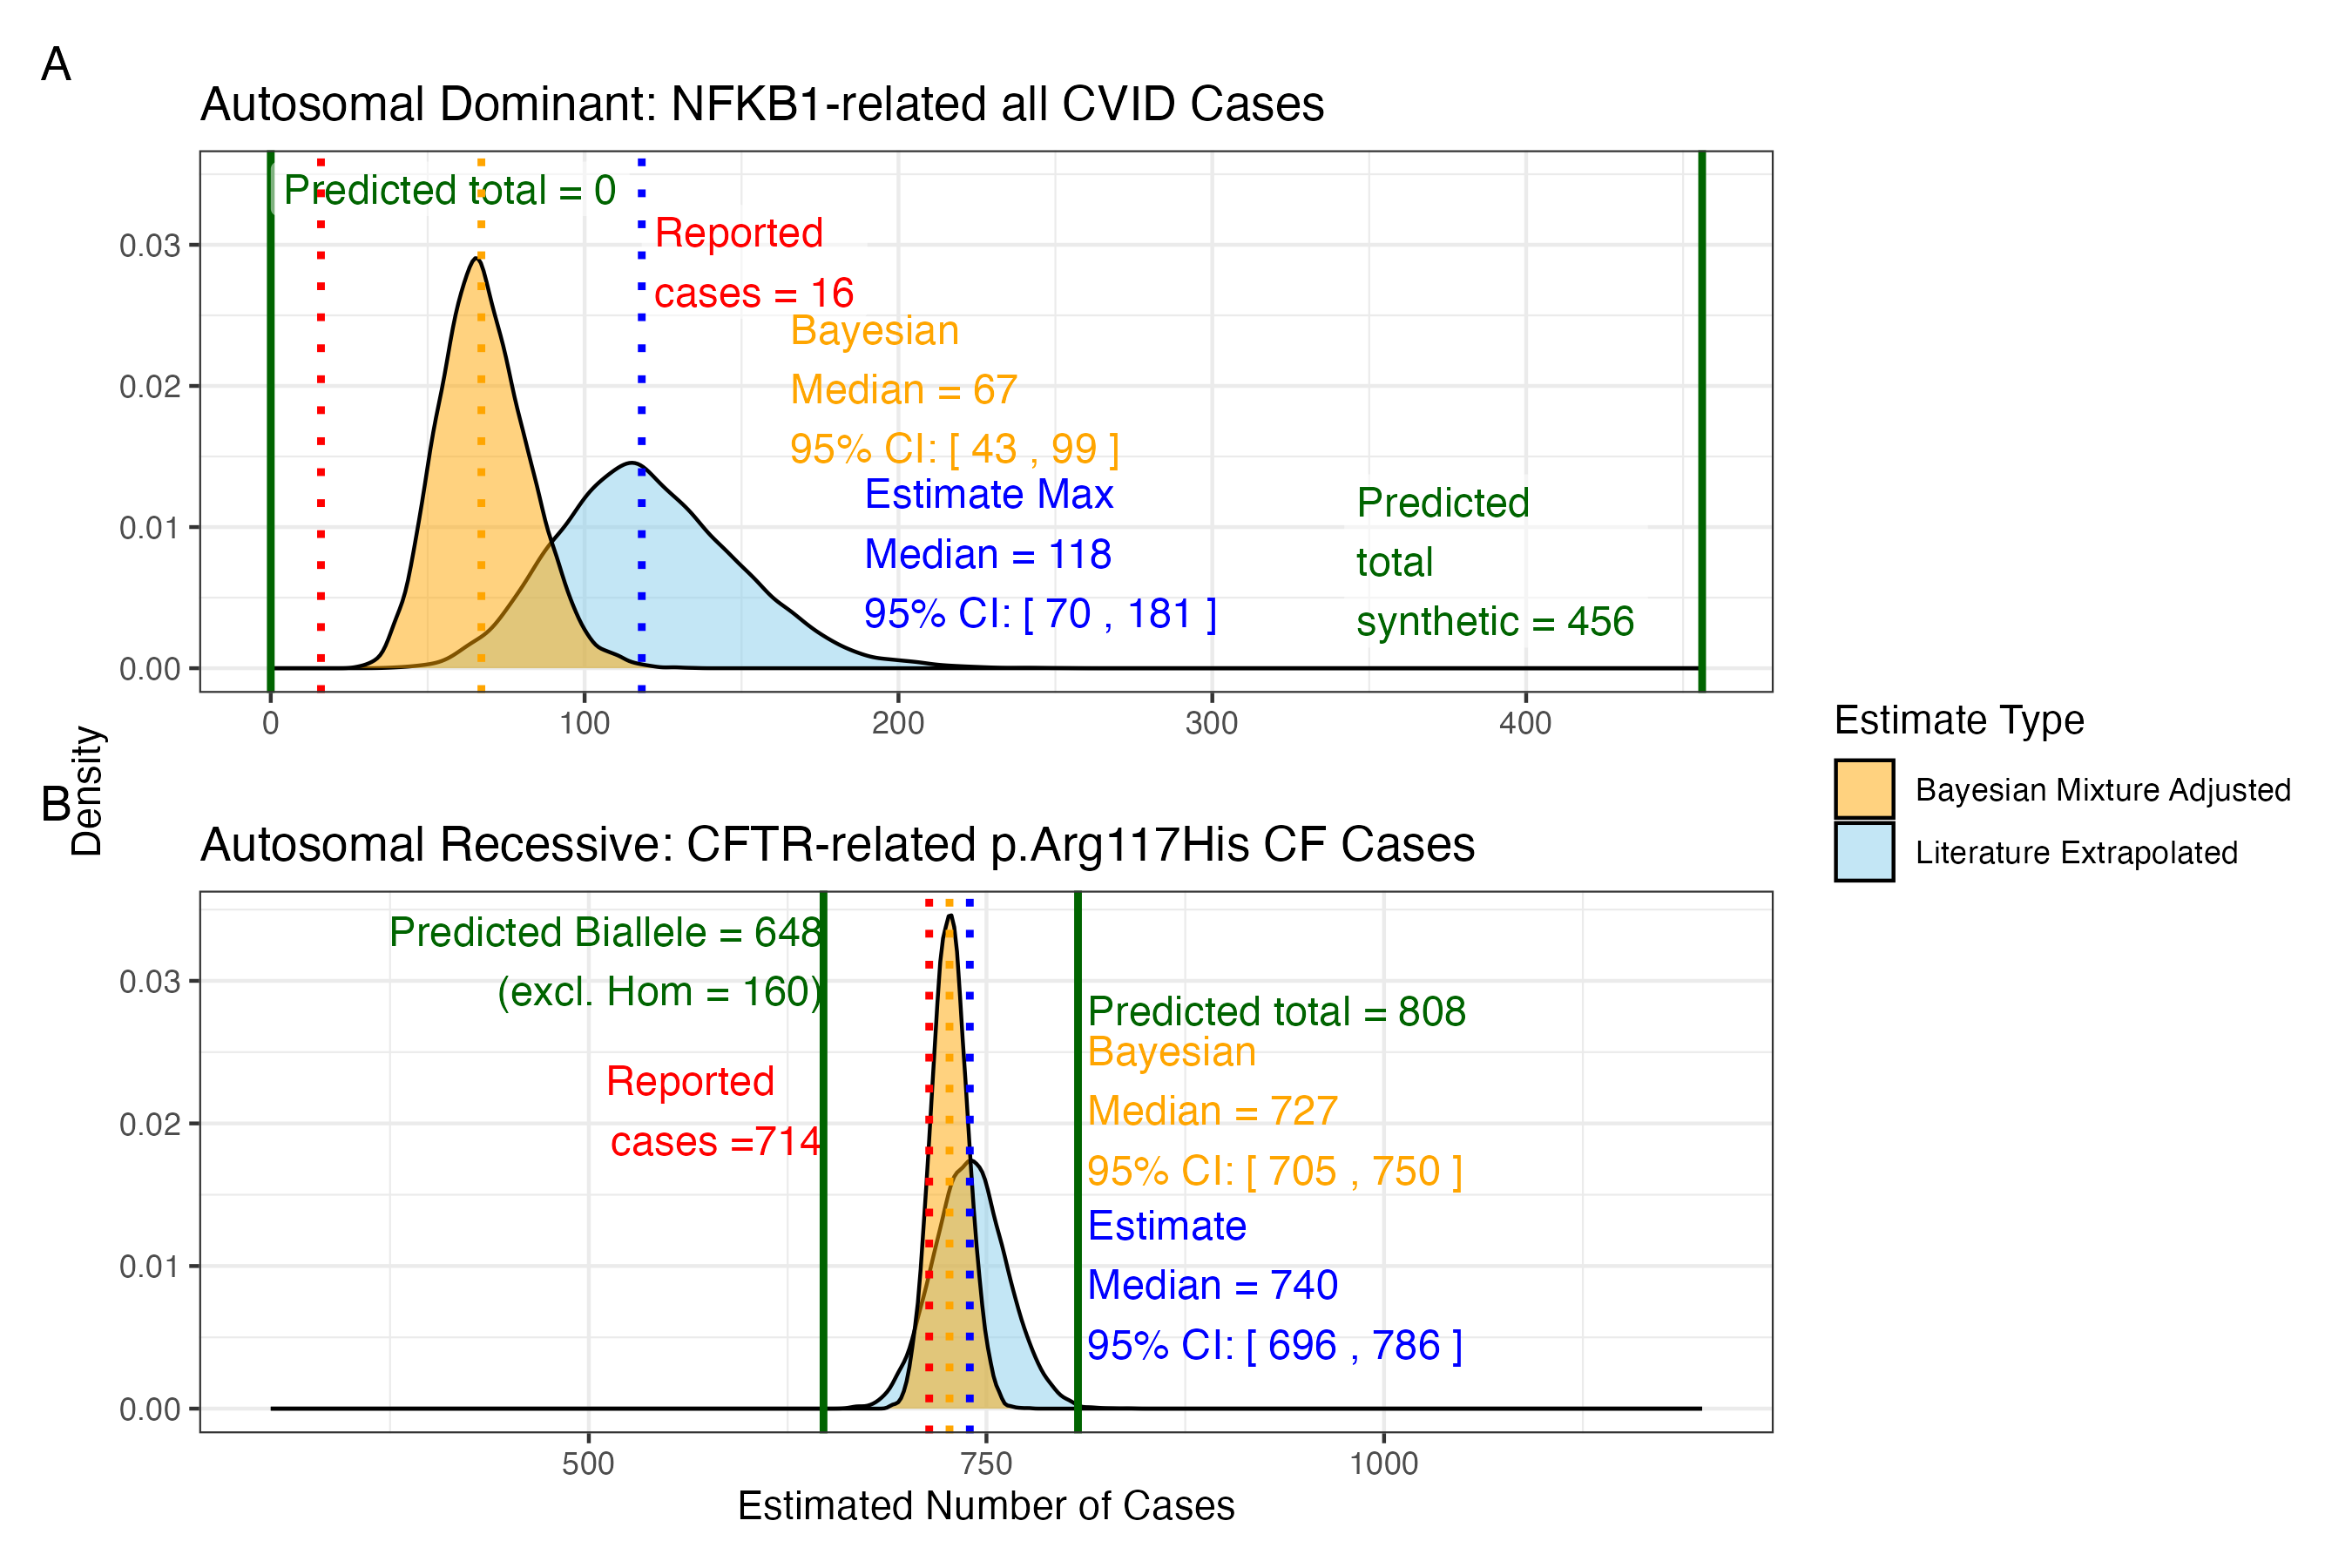
\includegraphics[width=0.99\textwidth]{../images/validation_studies_bayesian_adjusted_estimates.png}
  \caption{\textbf{Prior probabilities compared to validation disease cohort metrics.}
  (A) Density distributions for the number of \textit{NFKB1}-related CVID cases in the UK. 
  Our model (green) predicted 456 cases, which falls between the observed cohort count (red) of 390 and the upper extrapolated values.
  The blue curve represents maximum count of 1280, and the orange curve shows the Bayesian-adjusted mixture estimate of 835. 
(B) Density distributions for \textit{CFTR}-related p.Arg117His CF cases. 
Our model (green) predicted 648 biallelic cases and 808 total cases.
The nationally reported case count (red) was 714.
The blue curve represents maximum extrapolated count of 740, and the orange curve shows the Bayesian-adjusted mixture estimate of 727. We observed close agreement among the reported disease cases and our integrated probability estimation framework.}
  \label{fig:validation_studies_bayesian_adjusted_estimates}
\end{figure}

The density-scatter plot (\textbf{Figure \ref{fig:validation_scatter_dense}}) shows the final values for these genes of interest in a given population size and phenotype. It reveals that an allele frequency threshold of approximately 0.000007 is required to observe a single heterozygous disease-causing variant carrier in the UK population for both genes. However, owing to the autosomal recessive inheritance pattern of \textit{CFTR}, this threshold translates into more than 100,000 heterozygous carriers, compared to only 456 carriers for the autosomal dominant gene \textit{NFKB1}. Note that this allele frequency threshold, being derived from the current reference population, represents a lower bound that can become more precise as public datasets continue to grow. This marked difference underscores the significant impact of inheritance patterns on population carrier frequencies and the observed disease prevalence.

\begin{figure}[ht]
  \centering
  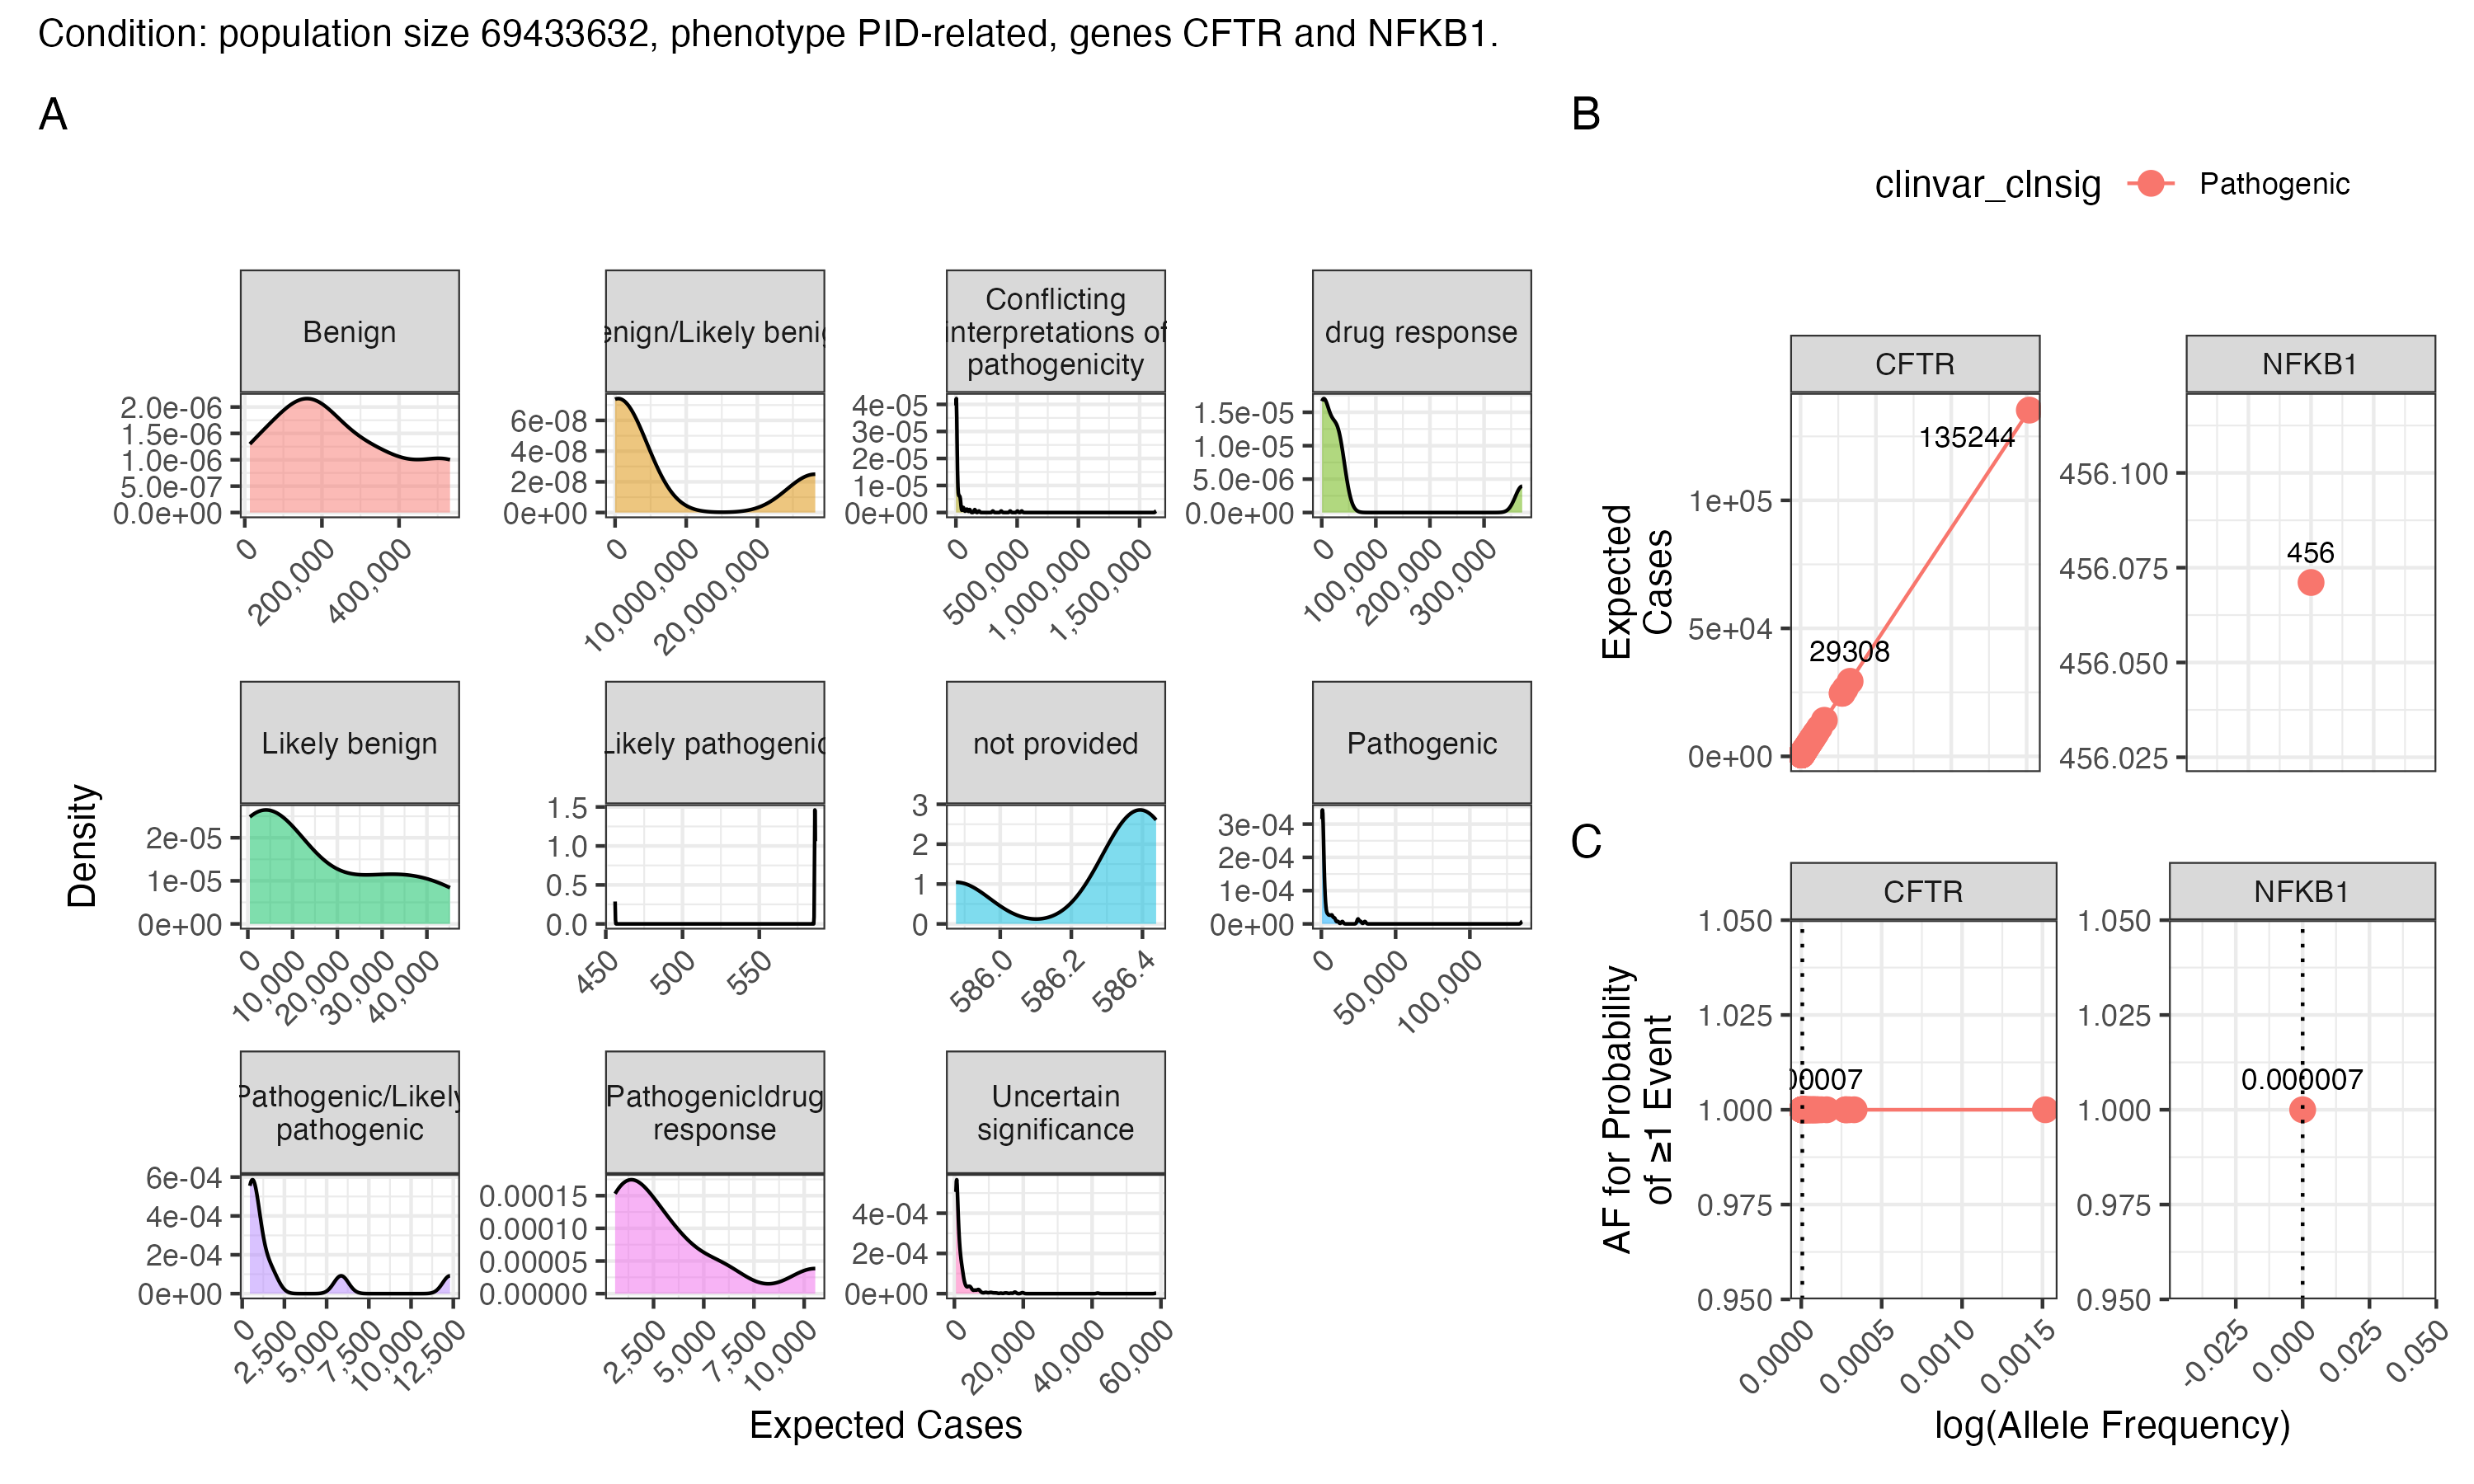
\includegraphics[width=\textwidth]{../images/validation_studies_scatterdense_expected_prob.png}
  \caption{\textbf{Interpretation of probability of observing a variant classification.} 
 The result from the chosen validation genes \textit{CFTR} and \textit{NFKB1} are shown. 
 Case counts are dependant on the population size and phenotype.
(A) The density plots of expected observations by ClinVar clinical significance. 
We then highlight the values for pathogenic variants specifically showing;
(B) the allele frequency versus expected cases in this population size and
(C) the probability of observing at least one event in this population size.}
  \label{fig:validation_scatter_dense}
\end{figure}

\subsection{Interpretation of ClinVar Variant Observations}

\textbf{Figure~\ref{fig:all_genes_combined_bar_charts_mini}} shows  the two validation study PID genes, representing autosomal recessive and dominant inheritance. \textbf{Figure~\ref{fig:all_genes_combined_bar_charts_mini} (A)}   illustrates the overall probability of an affected birth by ClinVar variant classification, whereas \textbf{Figure~\ref{fig:all_genes_combined_bar_charts_mini}  (B)}  depicts the total expected number of cases per classification for an example population, here the UK, of approximately 69.4 million. 

%While true positive pathogenic variants are typically straightforward to confirm, benign variants or variants of uncertain significance (VUS) may be overemphasized if their interpretation relies solely on the prominence of the associated gene. A variant may seem clinically significant simply because it occurs in a well-known gene, even if its empirical occurrence probability is high, suggesting that it is benign. This view underscores the necessity of considering the prior probability of variant occurrence when assessing pathogenicity.

\begin{figure}[ht]
  \centering
  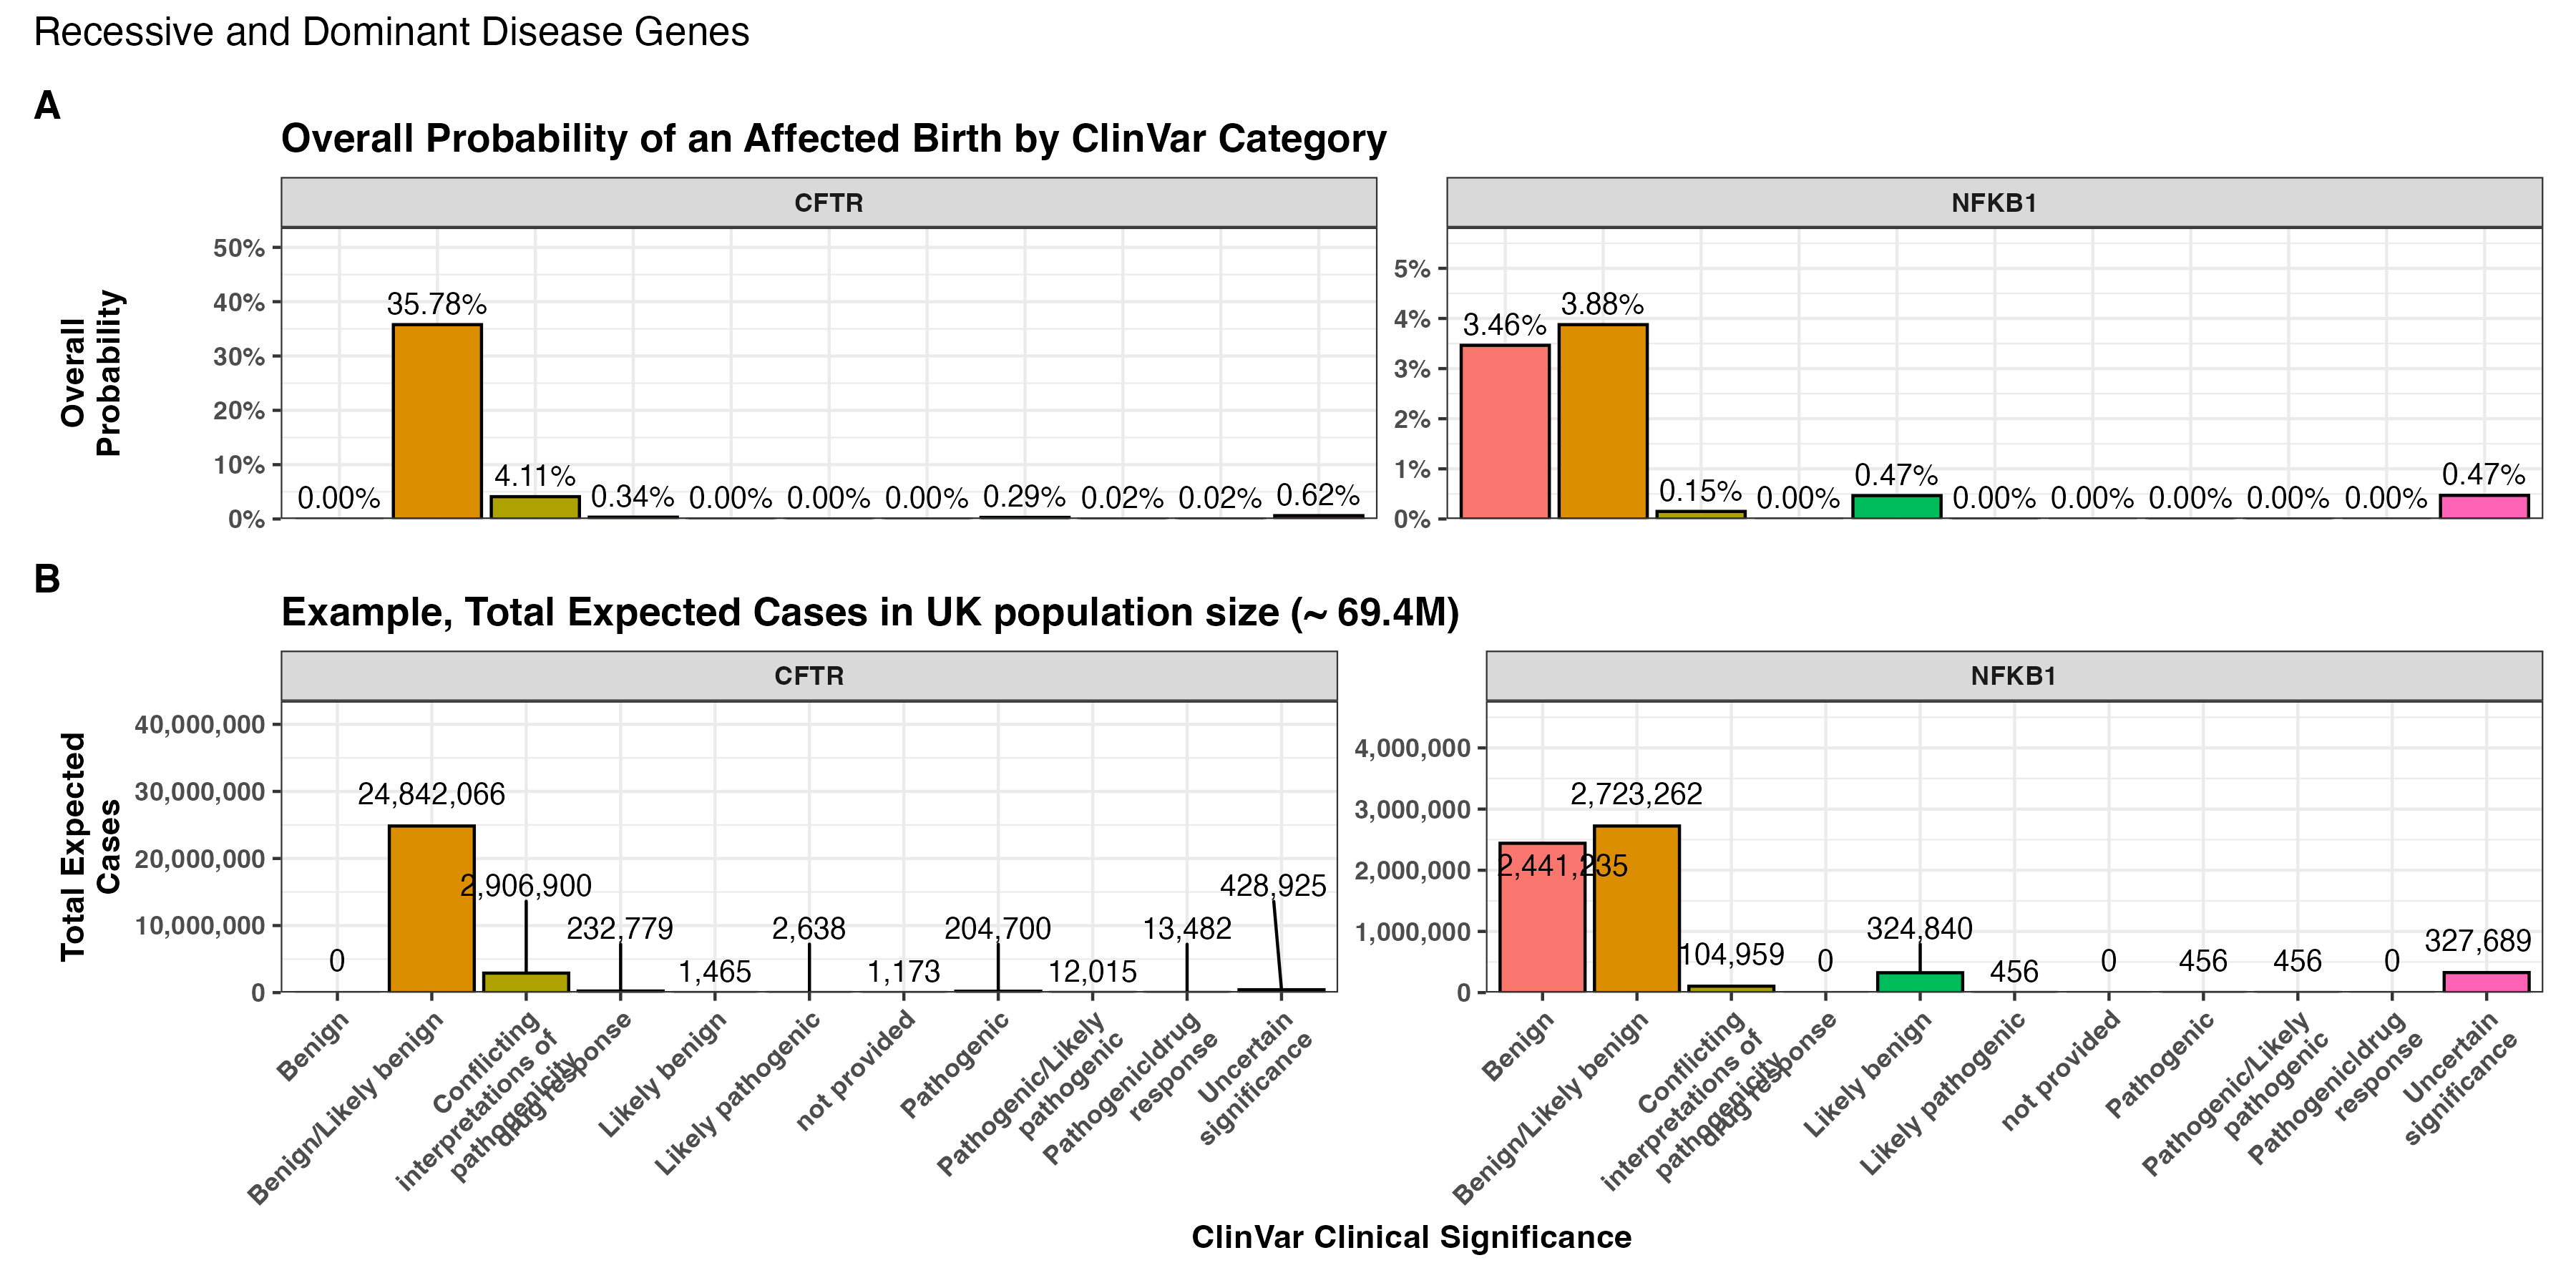
\includegraphics[width=0.99\textwidth]{../images/all_genes_combined_bar_charts_mini.png}
  \caption{\textbf{Combined bar charts summarizing the genome-wide analysis of ClinVar clinical significance for the PID gene panel}. Panel (A) shows the overall probability of an affected birth by variant classification, and (B) displays the total expected number of cases per classification, both stratified by gene. These integrated results illustrate the variability in variant observations across genes and underpin our validation of the probability estimation framework.}
  \label{fig:all_genes_combined_bar_charts_mini}
\end{figure}

\FloatBarrier

%\subsection{Genetic constraint in high-impact protein networks}
%\subsubsection{Overview of the PPI Network and Hub Gene Identification} 
%
%Describes the network visualisation where node size and colour reflect interaction degree and variant scores, and hub genes are labelled.
%
%The PPI network in \textbf{Figure \ref{fig:ppi_network_assoc} (A)}
%visually represents the complex interaction patterns among the genes in this disease panel, where nodes with higher log-transformed score-positive-total appear larger and red in colour.
%Unsurprisingly, the network of PPI is highly dense since these genes share many protein interactions. 
%
%
%
%\begin{figure}[ht]
%  \centering
%  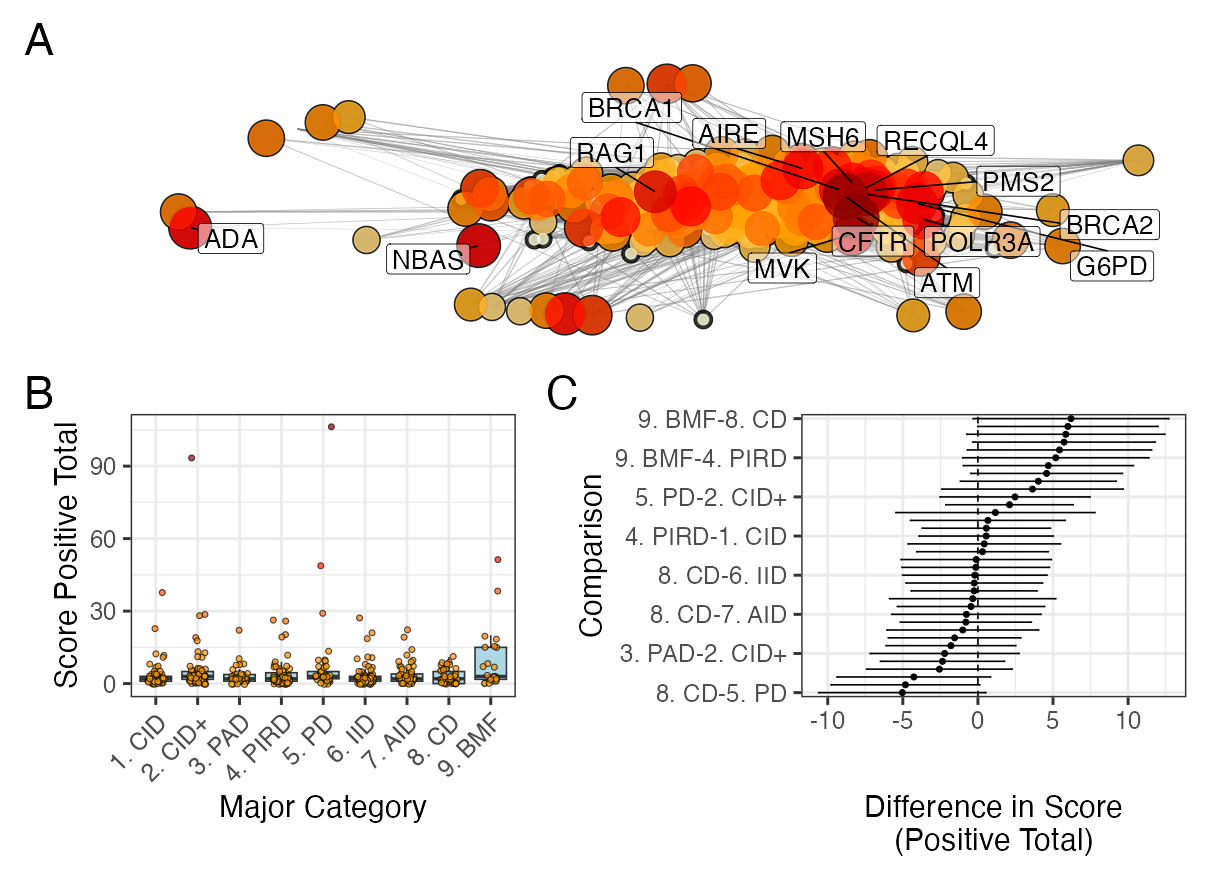
\includegraphics[width=\textwidth]{../images/untangleR_ppi_network_assoc_patch1.jpg}
%  \caption{
%    (A) Protein-protein interaction network among selected genes. Node size and colour reflect log-transformed score-positive-total values, with the top 15 nodes labelled.
%   (B) Boxplot with overlaid jittered points showing the distribution of score-positive-total across major disease categories.
%  (C) Tukey HSD post hoc comparisons of mean differences in score-positive-total between disease categories; intervals crossing zero indicate non-significant differences. Every 5th label shown on y-axis.
%  Alternate:
%    \textbf{ Network Graph of Selected Genes (p\_net).} 
%    This network graph was generated from STRING interaction data for a subset of genes.
%     Node sizes are scaled according to the normalized interaction degree, and node colours reflect the variant score (log-transformed \texttt{score\_positive\_total}). 
%    Labels indicate hub genes (those with degree in the top 5\textsuperscript{th} percentile). 
%    \textbf{Results:} Figure 1 illustrates the connectivity among the selected genes. Hub genes, which are crucial for network integrity, are labelled. The combined use of node size and colour provides insight into both interaction density and variant scores.}
%  \label{fig:ppi_network_assoc}
%\end{figure}

\subsection{Genetic constraint in high-impact protein networks}
\subsubsection{Overview of the PPI network and hub gene identification}

The ClinVar classifications reported in 
Figure \ref{fig:p_varRisEst_summary_scores} are scale -5 to +5 based on their pathogenicity. 
We were interested in positive (damaging) but not negative (benign) scoring variants, which are incidental to subsequent analysis. 
We tallied gene-level positive scores to give the score positive total metric. 
\textbf{Figure \ref{fig:ppi_network_assoc} (A)} shows the PPI network of disease-associated genes, where node size and colour encode the score positive total (log-transformed). 
The top 15 genes with the highest total prior probabilities of being observed with disease are labelled.

\begin{figure}[ht]
  \centering
  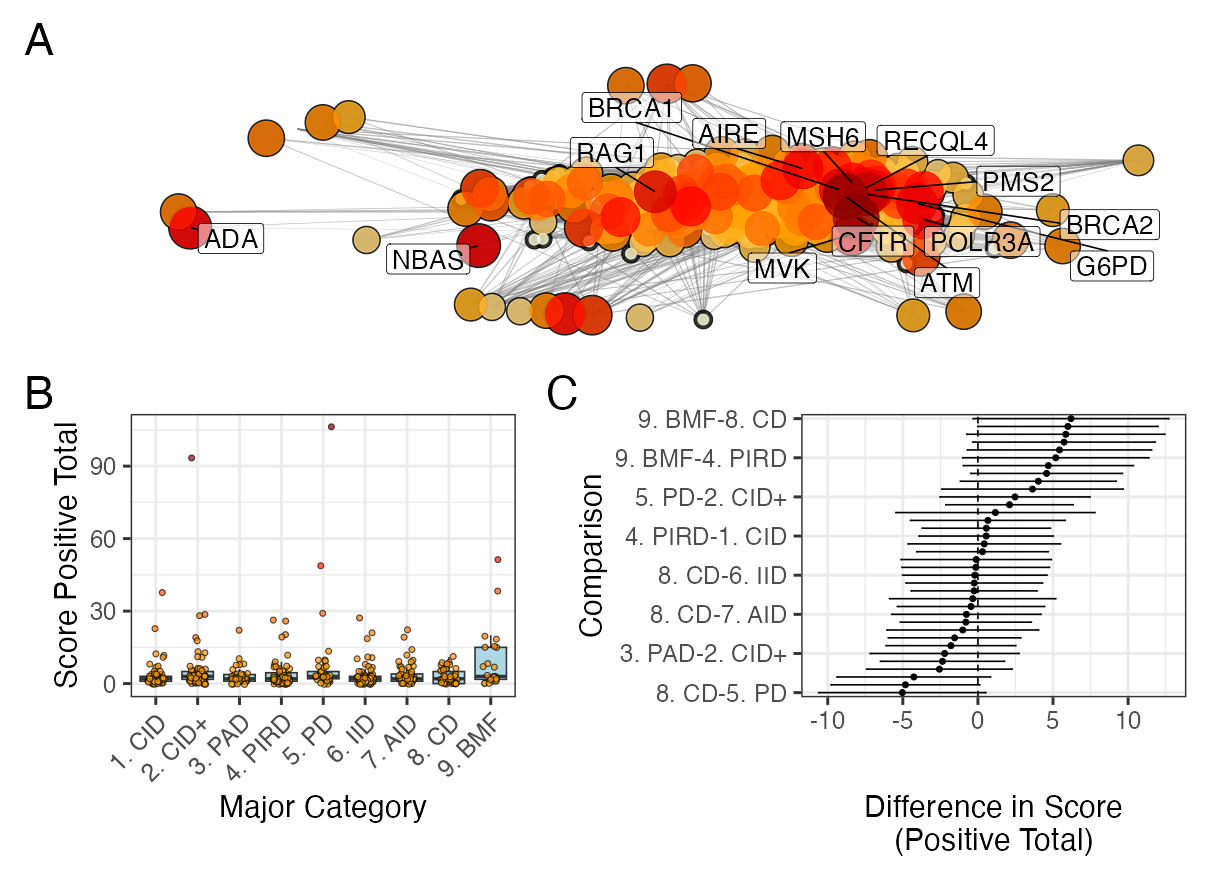
\includegraphics[width=\textwidth]{../images/untangleR_ppi_network_assoc_patch1.jpg}
  \caption{\textbf{PPI network and score positive total ClinVar significance variants}.
    (A) PPI network of disease-associated genes. Node size and colour represent the log-transformed \texttt{score\_positive\_total}, the top 15 genes/proteins with the highest probability of being observed in disease are labelled.
    (B) Distribution of \texttt{score\_positive\_total} across the major IEI disease categories.
    (C) Tukey HSD comparisons of mean differences in \texttt{score\_positive\_total} among all pairwise disease categories. Every 5th label is shown on y-axis.
  }
  \label{fig:ppi_network_assoc}
\end{figure}

\FloatBarrier
\subsubsection{Association Analysis of Score-Positive-Total across PID Categories} 

We checked for any statistical enrichment in score positive totals, which represents the expected observation of pathogenicity, between the IEI categories.
The one‐way ANOVA revealed an effect of major disease category on \texttt{score\_positive\_total} (\(F(8,500)=2.82,\,p=0.0046\)), indicating that group means are not identical, which we observed in
\textbf{Figure \ref{fig:ppi_network_assoc} (B)}.
However, despite some apparent differences in median scores across categories (i.e. 9. BMF), the Tukey honest significance test (HSD) post hoc comparisons 
\textbf{Figure \ref{fig:ppi_network_assoc} (C)}
showed that all pairwise differences had 95\% confidence intervals overlapping zero, suggesting that individual group differences were not significant.

\FloatBarrier
%\subsubsection{UMAP Embedding of the Protein-Protein Interaction Network} 
%Explains the dimensionality reduction (Figure 4) that reveals spatial gene clusters with dual labelling for hub genes and high variant score genes.
%
%- \textbf{Figure \ref{fig:p_umap}:} The UMAP embedding (p\_umap) effectively reduces the dimensionality of the PPI network, revealing spatial clusters of genes. The dual labelling strategy highlights both hub genes and genes with the highest variant scores, emphasizing key nodes that may warrant further investigation.
%
%In the UMAP it is interesting that genes with the highest total of positive variant classificaiton scores (i.e. more known pathogenic load) are distinctly separated from genes which have the highest interaction degree.
%Perhaps genes with high PPI degree cannot tollerate LOF which could affect a large netowrk of PID-realated genes, and thus selection has only tolerated the background allale frequency of damaging variants in genes with lower PPI degree since their effect is more specific consequences. 

%\subsubsection{UMAP Embedding of the Protein-Protein Interaction Network}
%To address the density of PPI of the IEI gene panel, we applied UMAP to the network
%as shown in 
%\textbf{Figure \ref{fig:p_umap}}. 
%The embedding separated the genes into automatically defined clusters.
%The interaction degree measures how strongly PPI connect proteins are connected based on the existing evidence.
%We were interested to test for Correlation between PPI Degree and the score positive total.
%\textbf{Figure \ref{fig:p_umap}} shows
%labelled the  nodes with the highest Degrees (above the 95th percentile) in blue color.
%The top 15 score positive total genes were labelled in yellow. 
%Notably, genes with high pathogenic variant loads segregate from highly connected nodes, suggesting that loss-of-function in hub genes was selectively constrained, whereas damaging variants in lower-degree genes yield more specific effects.
%We subsequently tested for this observation empirically.
%
%\begin{figure}[ht]
%  \centering
%  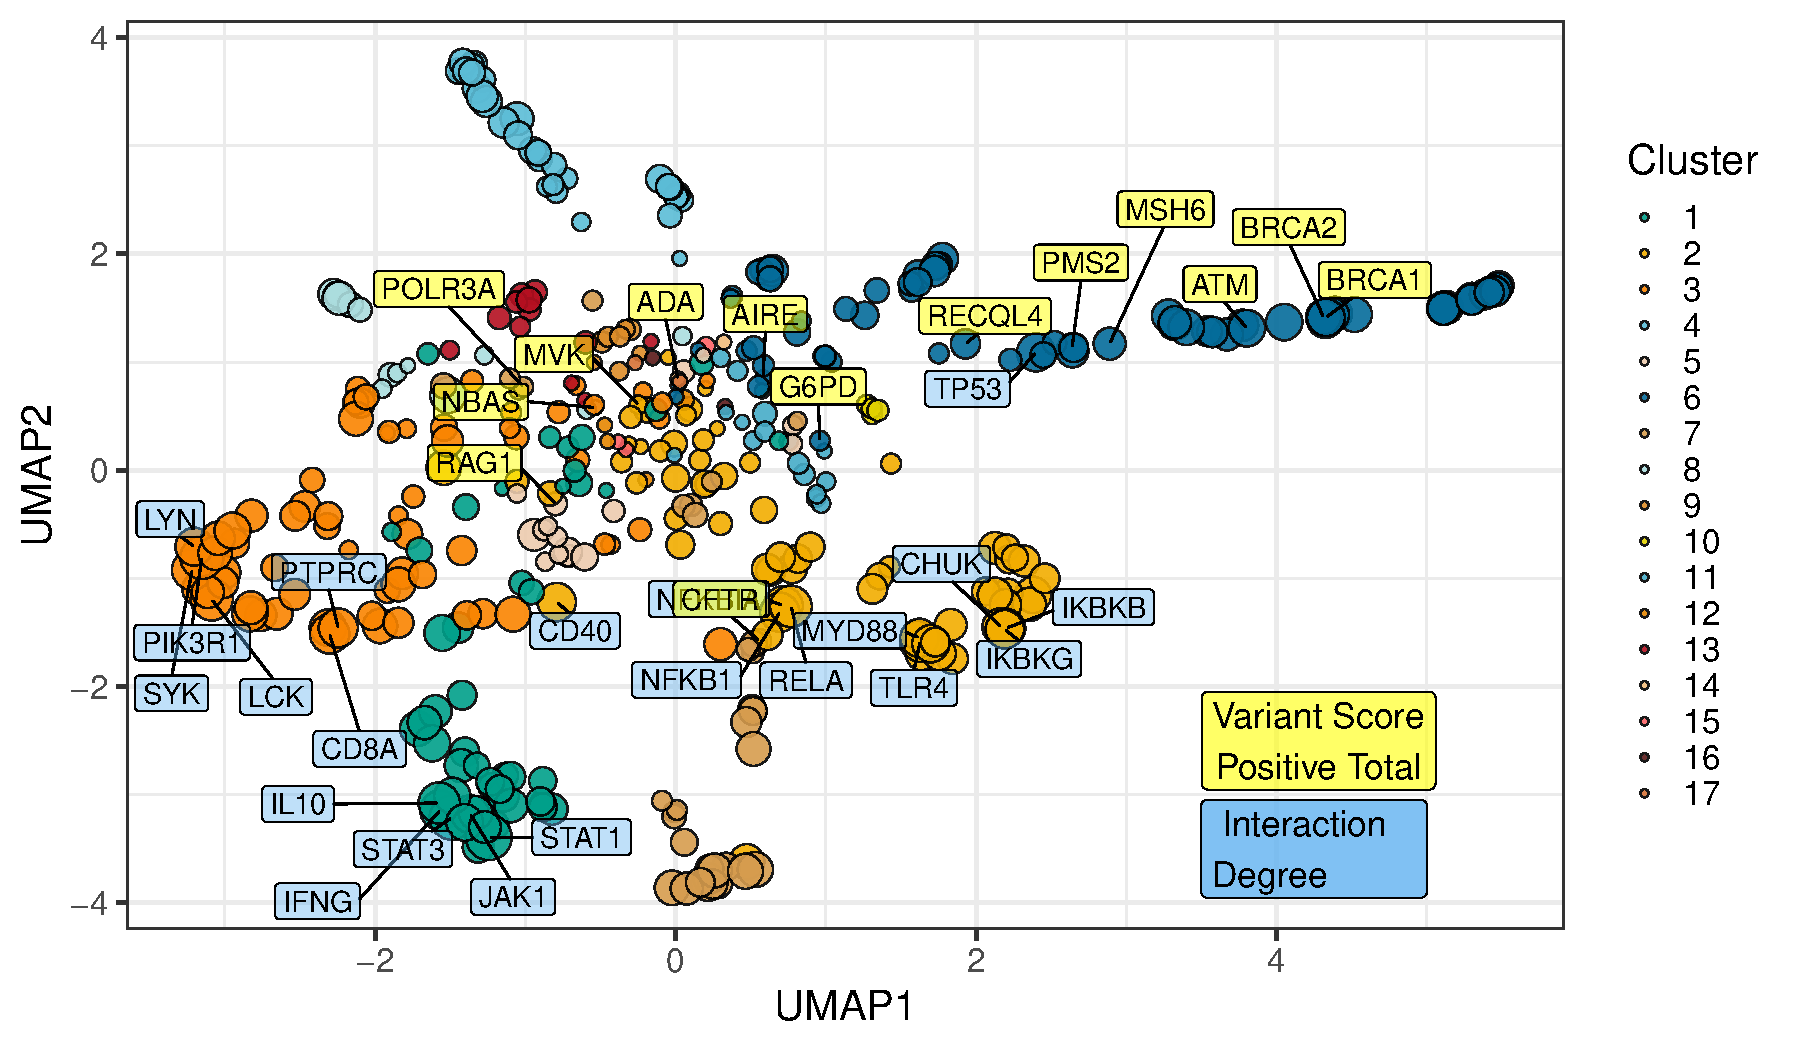
\includegraphics[width=0.99\textwidth]{../images/untangleR_ppi_network_umap.pdf}
%  \caption{
%    \textbf{Figure 4. UMAP Embedding of the PPI Network (p\_umap).}
%    This UMAP plot projects the high-dimensional protein-protein interaction network into two dimensions. Nodes are coloured by their assigned cluster using custom colours, and their sizes reflect interaction degree. Two sets of labels are included: blue labels denote hub genes (high interaction degree) and yellow labels highlight the top 15 genes based on \texttt{score\_positive\_total}.
%    \textbf{Results:} The UMAP embedding in Figure 4 facilitates the visual identification of network clusters. Dual labelling helps pinpoint key genes that are either highly connected or have high variant scores, offering insights into potential drivers of the observed network structure.
%  }
%  \label{fig:p_umap}
%\end{figure}
%





\subsubsection{UMAP Embedding of the Protein-Protein Interaction Network}
To address the density of the PPI network for the IEI gene panel, we applied UMAP (\textbf{Figure \ref{fig:p_umap}}). The embedding automatically defined gene clusters. Node sizes reflect interaction degree, a measure of evidence-supported connectivity. We tested for a correlation between interaction degree and \texttt{score\_positive\_total}. In \textbf{Figure \ref{fig:p_umap}}, nodes with degrees above the 95th percentile are labelled in blue, while the top 15 genes by \texttt{score\_positive\_total} are labelled in yellow. Notably, genes with high pathogenic variant loads segregate from highly connected nodes, suggesting that loss-of-function in hub genes is selectively constrained, whereas damaging variants in lower-degree genes yield more specific effects. This observation was subsequently tested empirically.

\begin{figure}[ht]
  \centering
  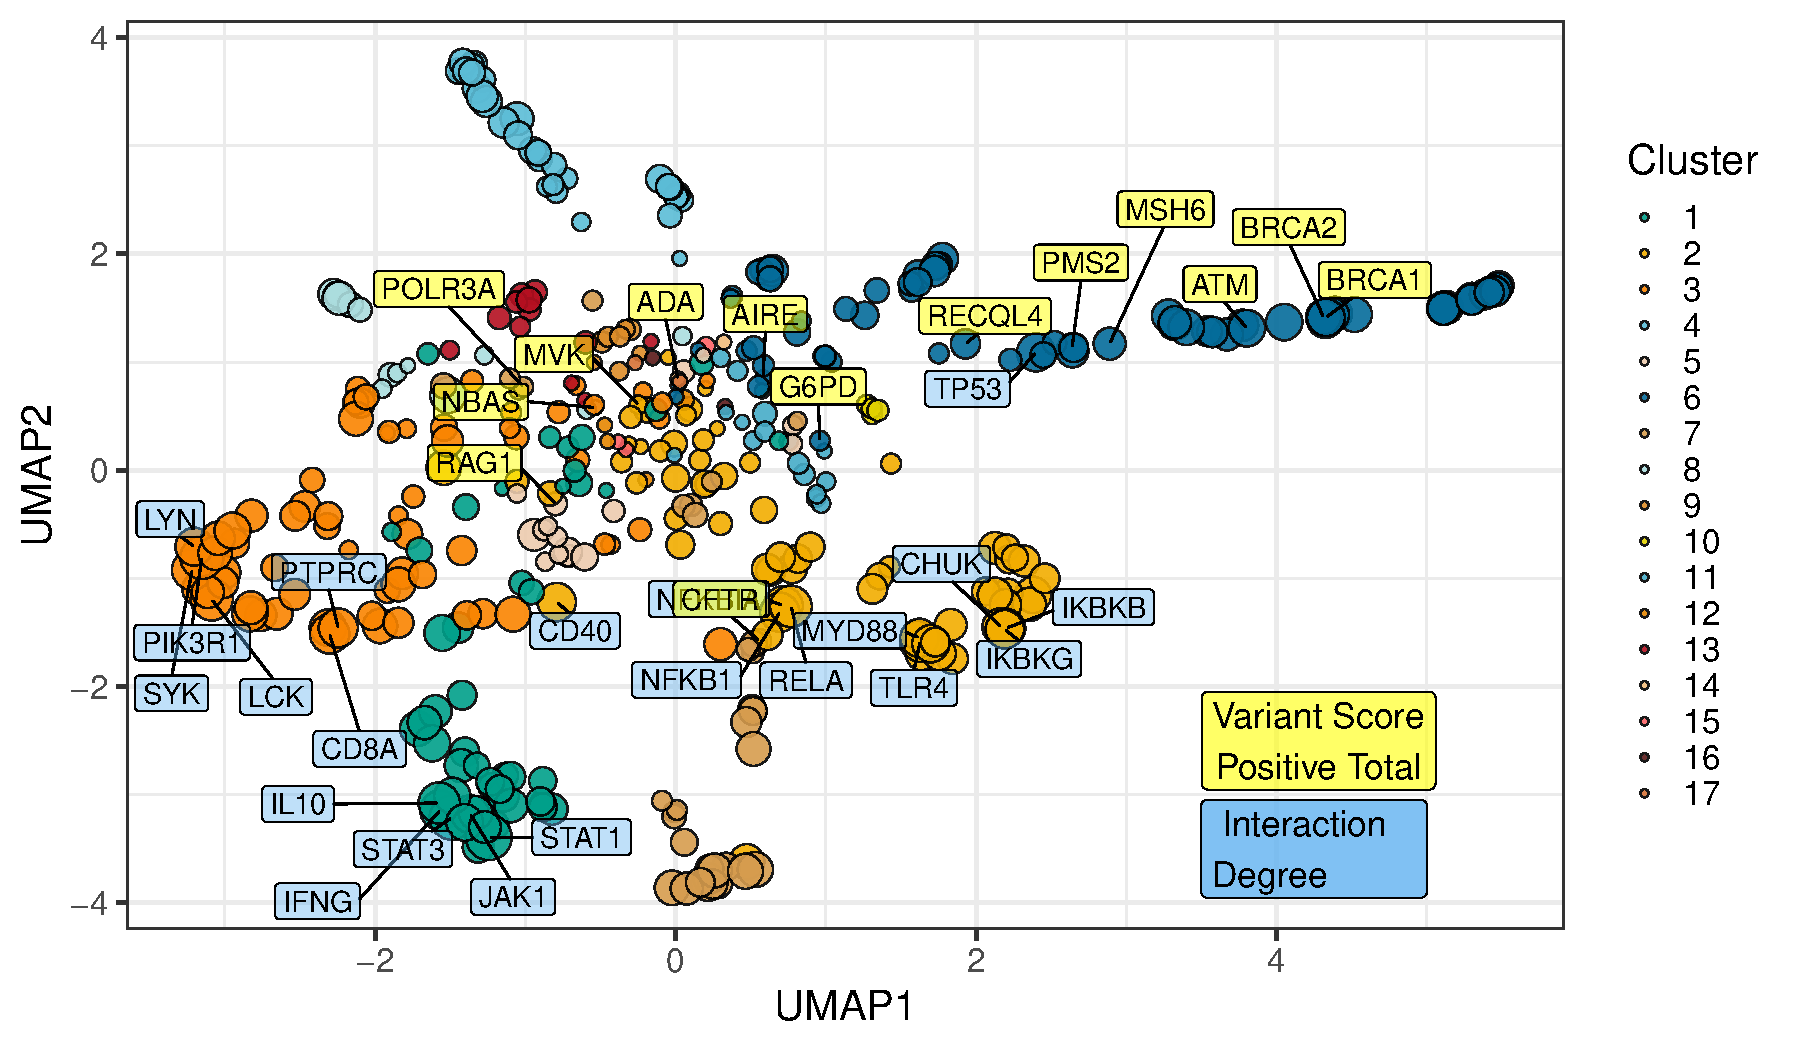
\includegraphics[width=0.99\textwidth]{../images/untangleR_ppi_network_umap.pdf}
  \caption{
    \textbf{UMAP embedding of the PPI network (p\_umap).} 
    The plot projects the high-dimensional protein-protein interaction network into two dimensions, with nodes coloured by cluster and sized by interaction degree. Blue labels indicate hub genes (degree above the 95th percentile) and yellow labels mark the top 15 genes by score positive total (damaging ClinVar classifications). The spatial segregation suggests that genes with high pathogenic variant loads are distinct from highly connected nodes.
  }
  \label{fig:p_umap}
\end{figure}



\FloatBarrier
%\subsubsection{Hierarchical Clustering of Enrichment Scores for Major Disease Categories} 
%Presents the clustered heatmap and dendrogram (Figure 3) showing enrichment patterns of disease categories across network clusters.
%
%% Figure 3: patch2
%\begin{figure}[ht]
%  \centering
%  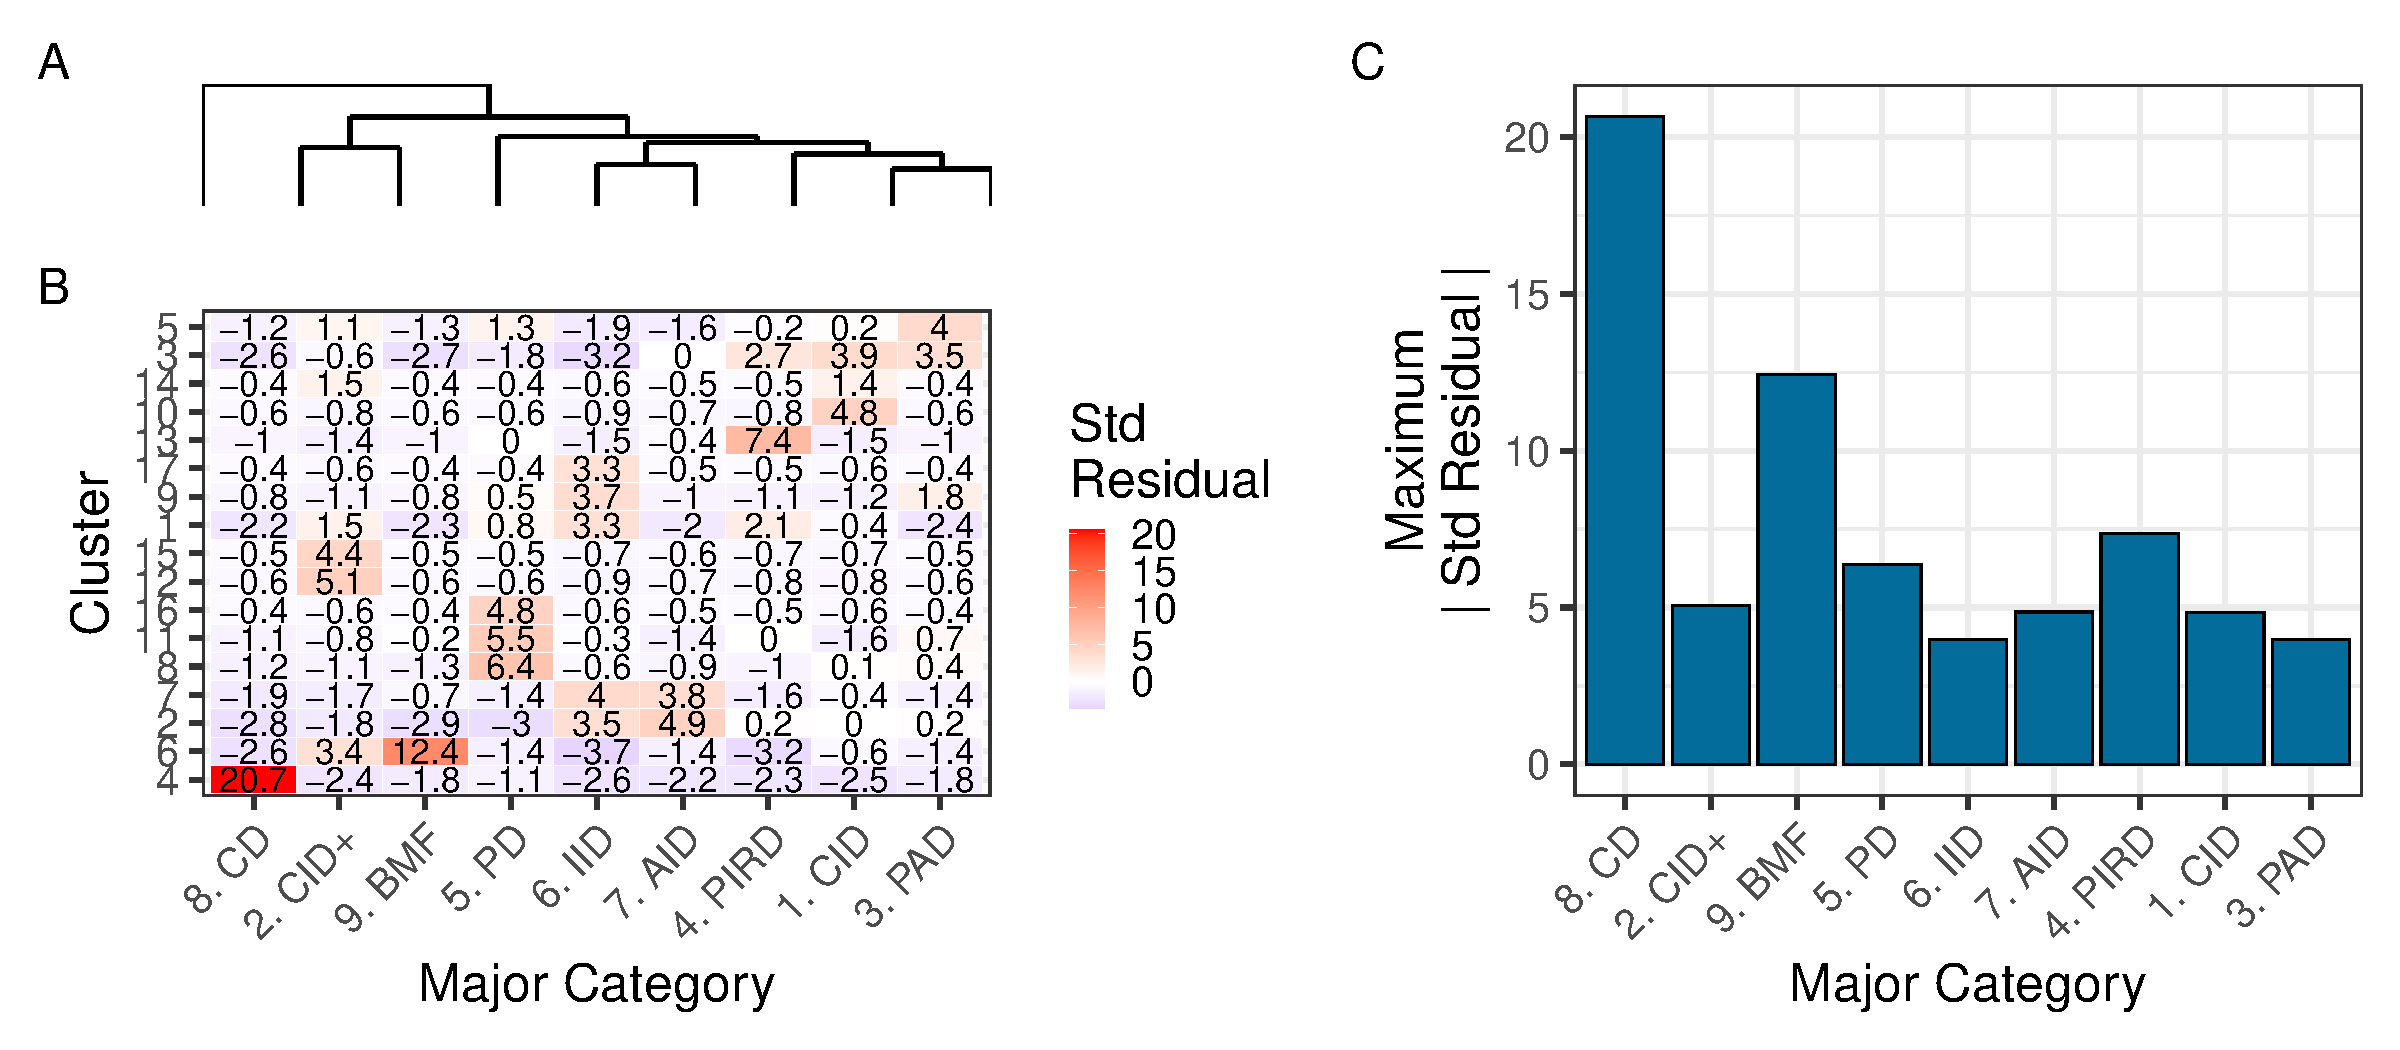
\includegraphics[width=0.99\textwidth]{../images/untangleR_ppi_network_patch2_cator.pdf}
%  \caption{
%    \textbf{Figure 3. Hierarchical Clustering of Enrichment Scores (patch2).} 
%    This figure presents a hierarchically clustered heatmap of standardized residuals (enrichment scores) for major disease categories by network cluster, accompanied by a dendrogram for the major categories and a bar plot indicating the maximum absolute enrichment per category. 
%    \textbf{Results:} Figure 3 reveals enrichment patterns across clusters; categories with absolute standardized residuals greater than 2 indicate significant enrichment or depletion. The dendrogram visually groups similar categories, highlighting potential biological relationships.}
%  \label{fig:patch2}
%\end{figure}

\subsubsection{Hierarchical Clustering of Enrichment Scores for Major Disease Categories}
\textbf{Figure \ref{fig:patch2}} presents a heatmap of standardised residuals for major disease categories across network clusters, as per \textbf{Figure \ref{fig:p_umap}}. A dendrogram clusters similar disease categories, while the accompanying bar plot displays the maximum absolute standardised residual for each category.
Notably, (8) complement deficiencies (CD) shows the highest maximum enrichment, followed by 
(9) Bone marrow failure (BMF). While all maximum values exceed 2, the threshold for significance, this likely reflects the presence of protein clusters with strong damaging variant scores rather than uniform significance across all categories (i.e. genes from cluster 4 in 8.CD).

%\FloatBarrier
%\subsubsection{Correlation between PPI Degree and LOEUF Constraint Metrics} 
%Summarises the Spearman correlation analysis between network connectivity and constraint (Figure 5A/B) and its variation across clusters.
%
%We first checked for any strong correlation between the cluster groups and constraint in supplemental Figure \ref{fig:p_umap_const} however no clear features were evident visually.
%
%\begin{figure}[ht]
%  \centering
%  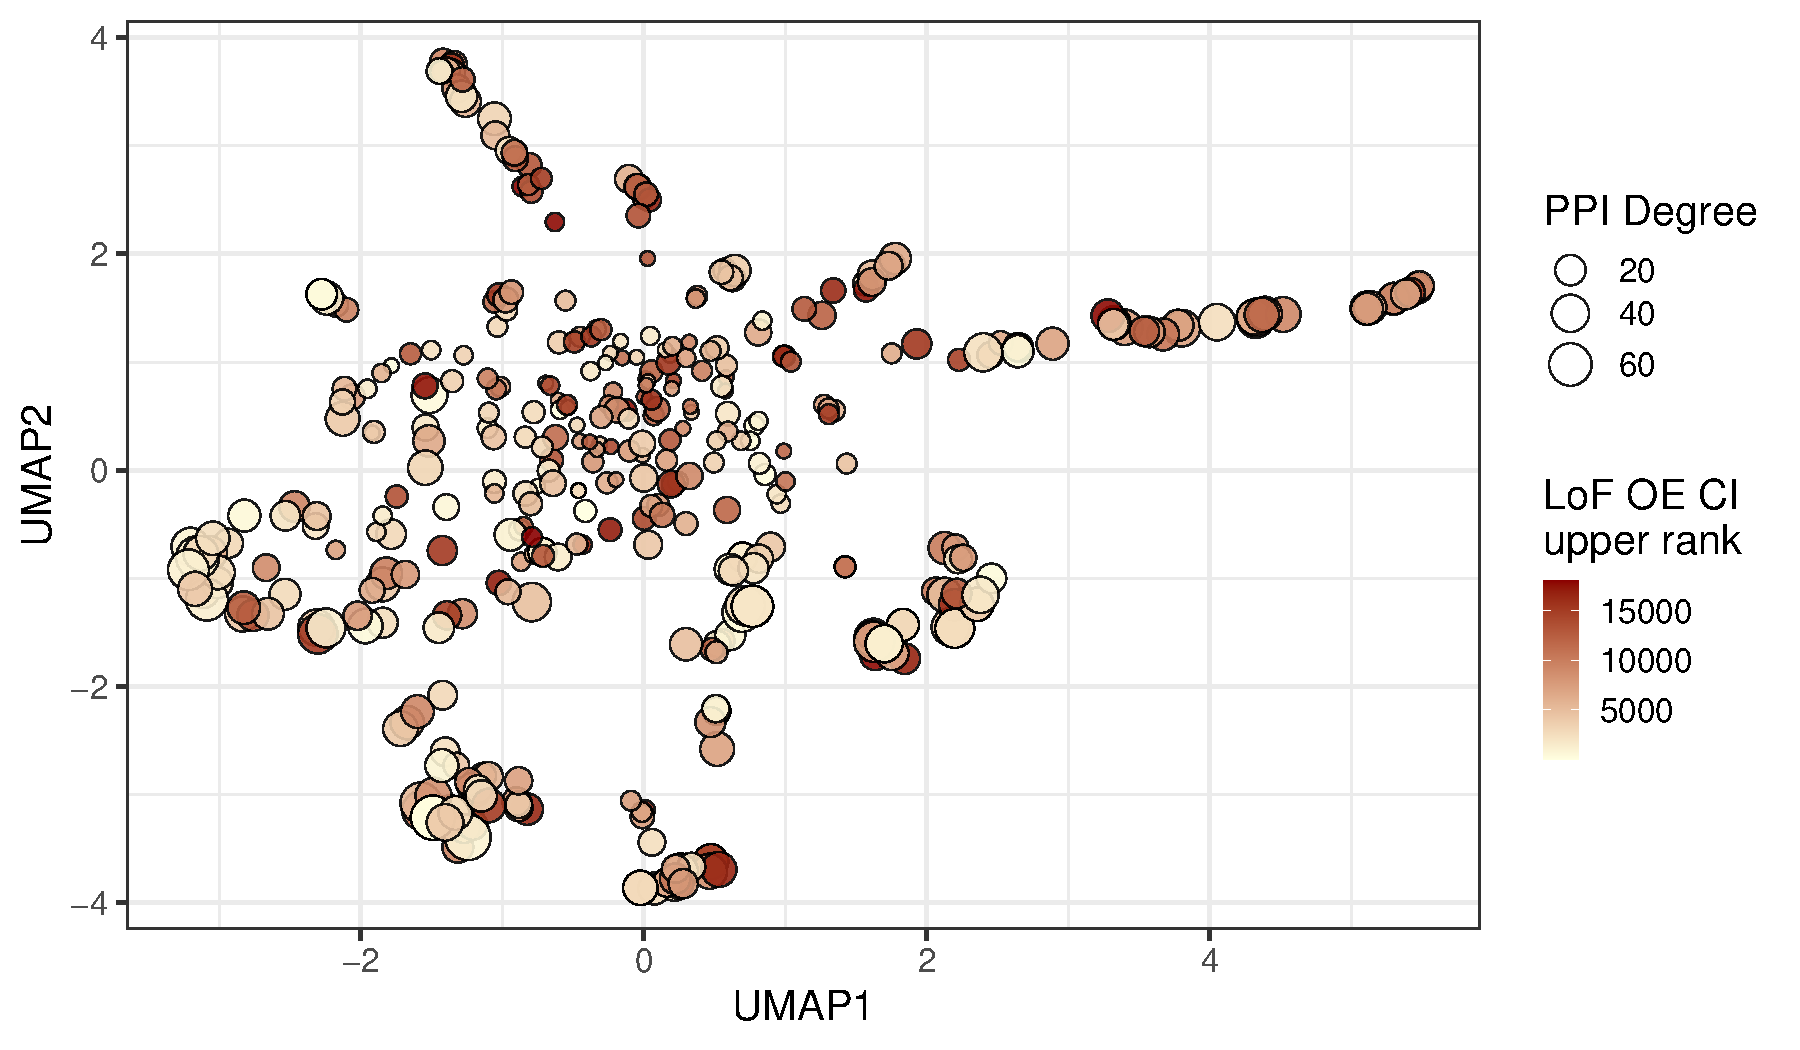
\includegraphics[width=0.99\textwidth]{../images/untangleR_ppi_network_p_umap_const.pdf}
%  \caption{ }
%  \label{fig:p_umap_const}
%\end{figure}
%
%Statistical analysis was used.
%Figure  \ref{fig:p_cor_spear_rho_sig_clust_patch3}:  The overall network analysis demonstrates a weak, significant negative correlation between PPI degree and LOEUF upper rank. However, when stratified by gene clusters, several clusters show stronger correlations, implying that the constraint on loss-of-function variation may be particularly pronounced in specific functional gene groups. Further investigation is needed to elucidate the biological underpinnings of these cluster-specific differences.
%
%
%\begin{figure}[ht]
%  \centering
%  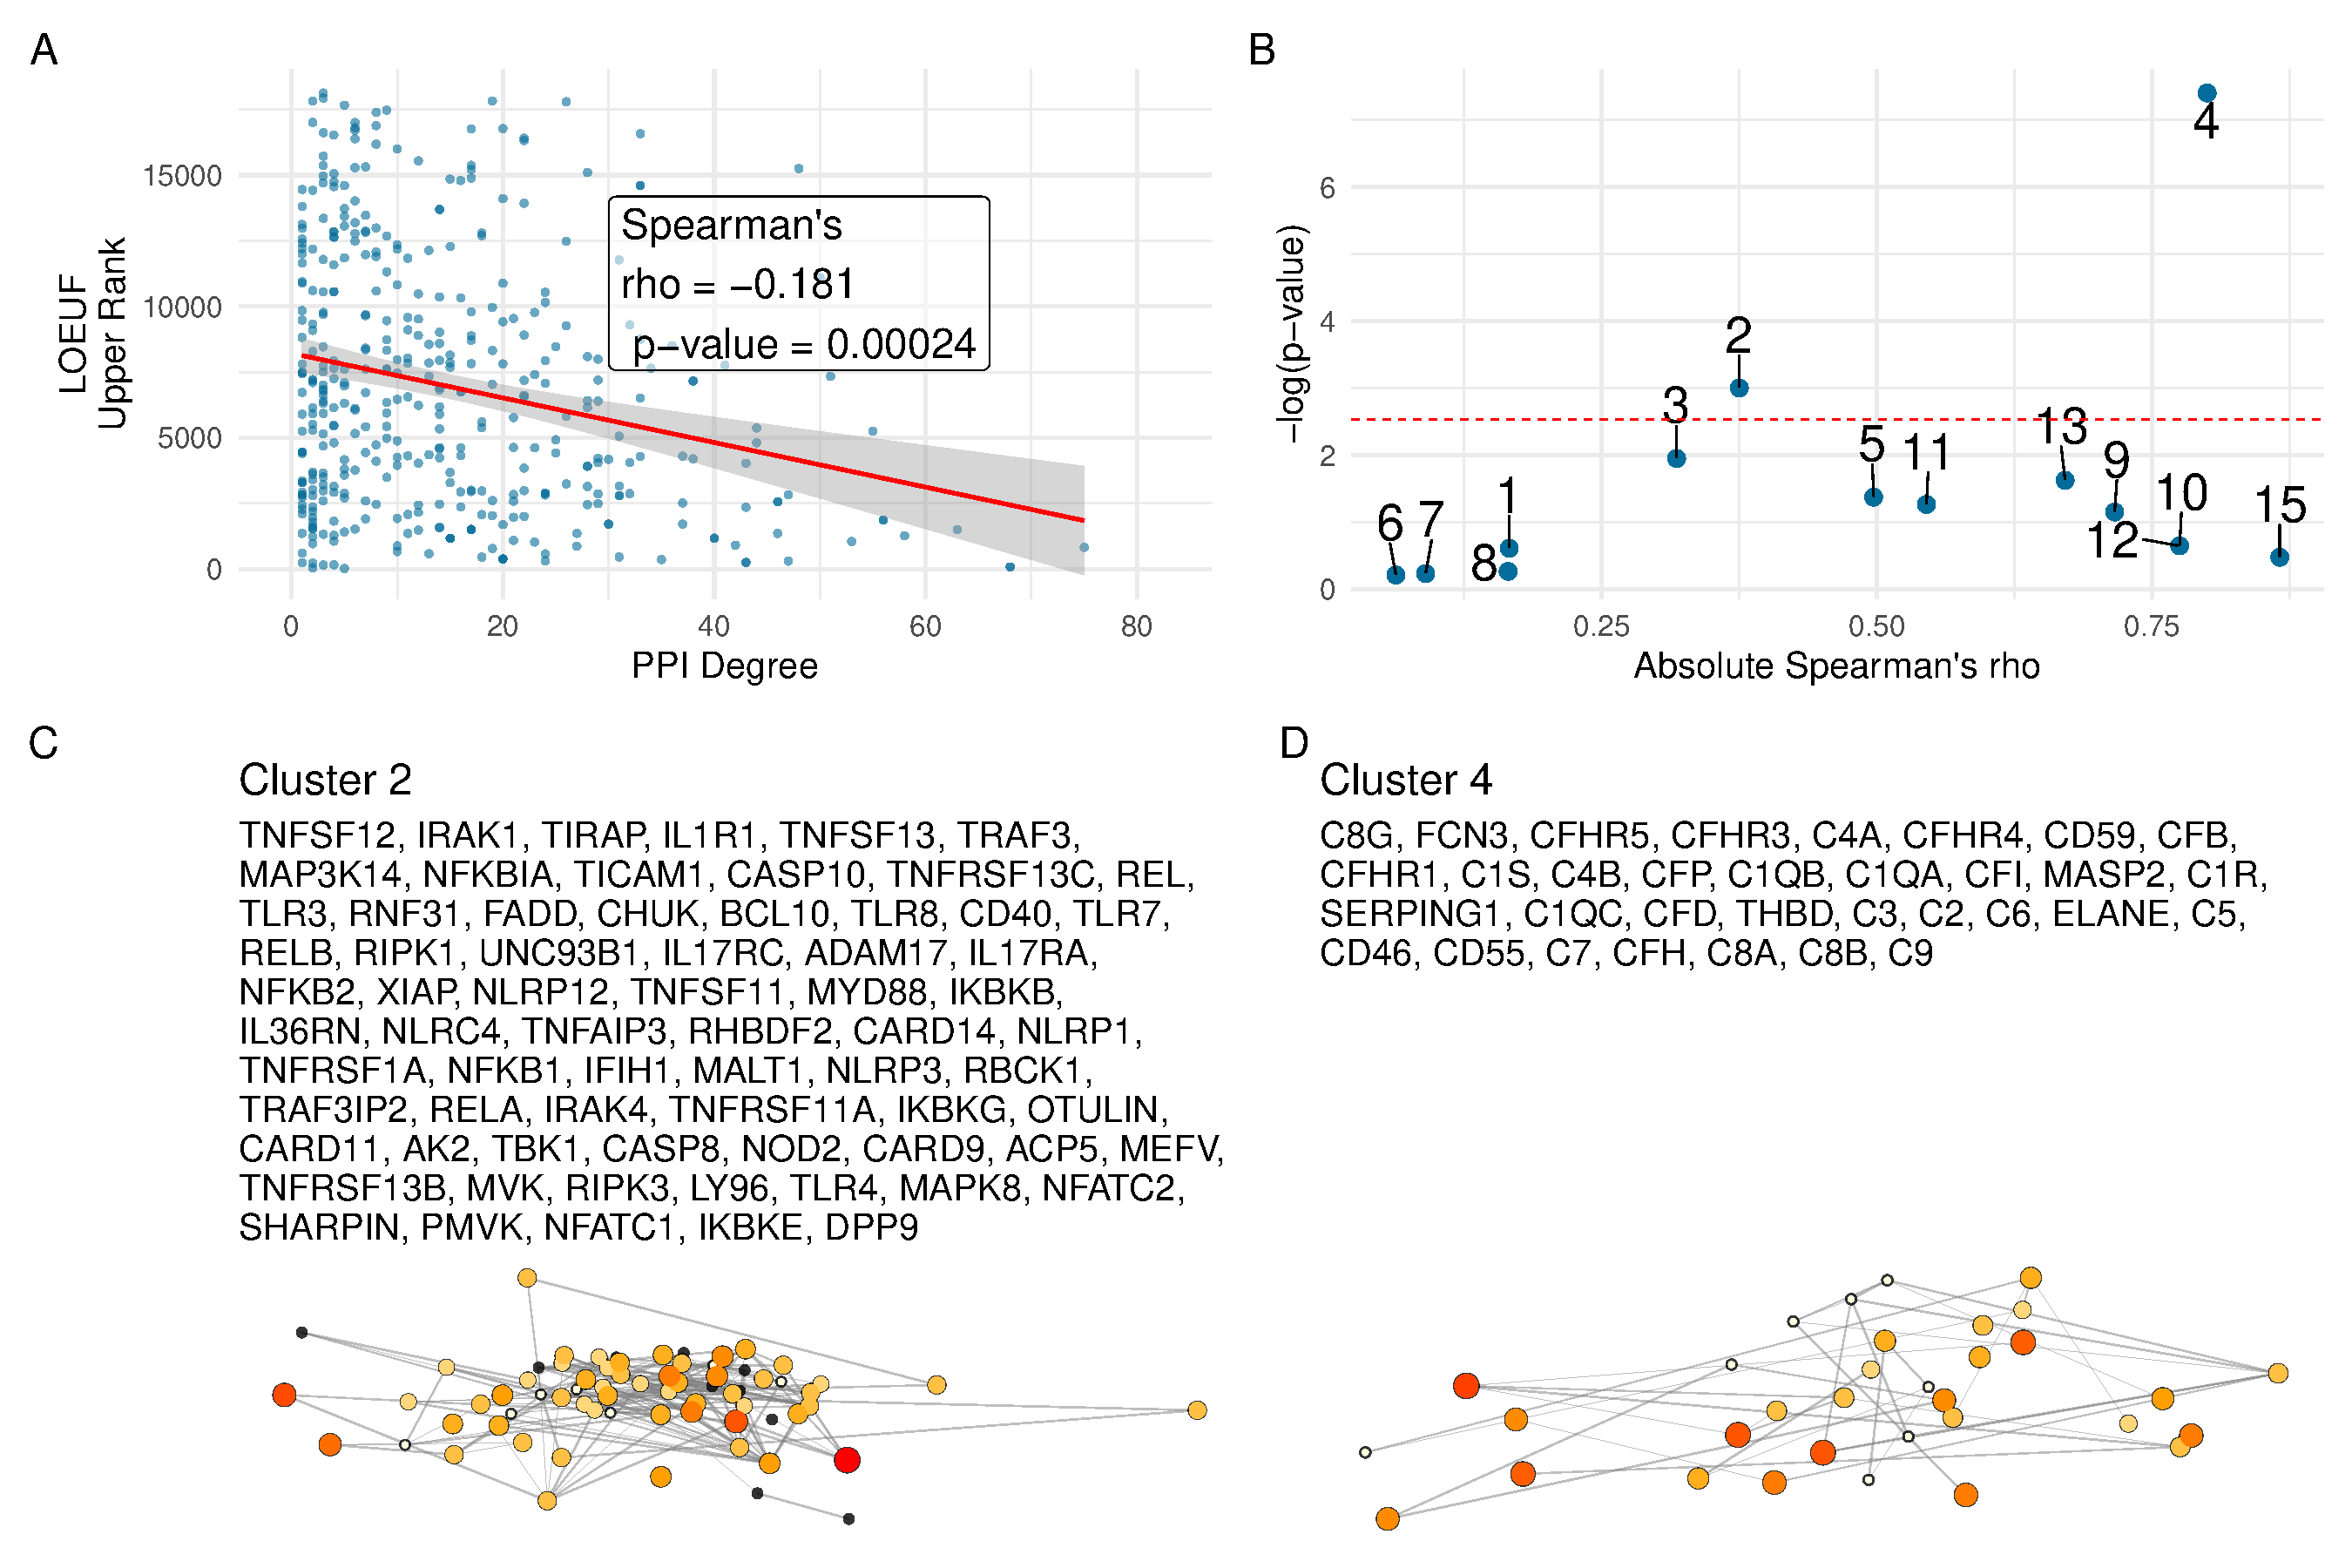
\includegraphics[width=0.99\textwidth]{../images/untangleR_ppi_network_p_cor_spear_rho_sig_clust_patch3.pdf}
%  \caption{
%    \textbf{(A) Scatter Plot and (B) Cluster-wise Correlation Analysis of PPI Degree vs. LOEUF Upper Rank.}
%    \textbf{(A)} The scatter plot shows the relationship between PPI degree and LOEUF upper rank for all genes in the network. A Spearman's rank correlation test yields ρ = –0.181 (p = 0.00024), indicating a weak but statistically significant negative correlation. This suggests that genes with higher connectivity tend to have lower LOEUF values (i.e. they are more constrained), consistent with the hypothesis that highly interactive genes are less tolerant of loss-of-function variants.
%    \textbf{(B)} The bar/scatter plot displays the absolute Spearman’s ρ values (converted to a positive scale) and the –log(p-value) for each cluster. Notably, clusters such as 2 (ρ = –0.375, p = 0.000994), 3 (ρ = –0.318, p = 0.0112), 4 (ρ = –0.800, p < 0.000001), and 5 (ρ = –0.497, p = 0.0423) show moderate to strong correlations, whereas other clusters (e.g. clusters 1, 6, 7, and 8) exhibit weak or non-significant relationships. These variations suggest that the association between connectivity and constraint differs markedly across functional gene groups.
%    \textbf{(C) and (D)}: Network plots of enriched significant clusters based on gnomAD constraint metrics. 
%  }
%  \label{fig:p_cor_spear_rho_sig_clust_patch3}
%\end{figure}

\subsubsection{PPI Connectivity, LOEUF Constraint and Enriched Network Cluster Analysis}
%\subsubsection{Correlation between PPI Degree and LOEUF Constraint Metrics}
We evaluated the relationship between network connectivity (PPI degree) and loss-of-function constraint (LOEUF upper rank) using Spearman’s rank correlation (see \textbf{Figure \ref{fig:p_cor_spear_rho_sig_clust_patch3}}). Overall, there is a weak but significant negative correlation (ρ = –0.181, p = 0.00024), indicating that highly connected genes tend to be more constrained. However, when stratified by gene clusters, some clusters (e.g. clusters 2, 3, 4, and 5) show moderate to strong correlations, whereas others (clusters 1, 6, 7, and 8) do not. These findings suggest that constraint on loss-of-function variation varies among functional gene groups.

We assessed the correlation between network connectivity and LOEUF constraint. 
A supplementary analysis (\textbf{Figure \ref{fig:p_umap_const}}) did not reveal distinct visual associations between network clusters and constraint metrics, possibly due to the high network density.
We therefore tested for correlation quantitatively. As shown in \textbf{Figure \ref{fig:p_cor_spear_rho_sig_clust_patch3}(A)}, there was a weak but significant negative Spearman correlation (ρ = –0.181, p = 0.00024) between PPI degree and LOEUF upper rank, suggesting that highly connected genes are more constrained. Notably, when stratified by clusters, the correlation is stronger in specific groups, clusters 2 (ρ = –0.375, p = 0.000994), 4 (ρ = –0.800, p < 0.000001), indicating that shared mechanisms within pathway clusters may accentuate genetic constraints.


\begin{figure}[ht]
  \centering
  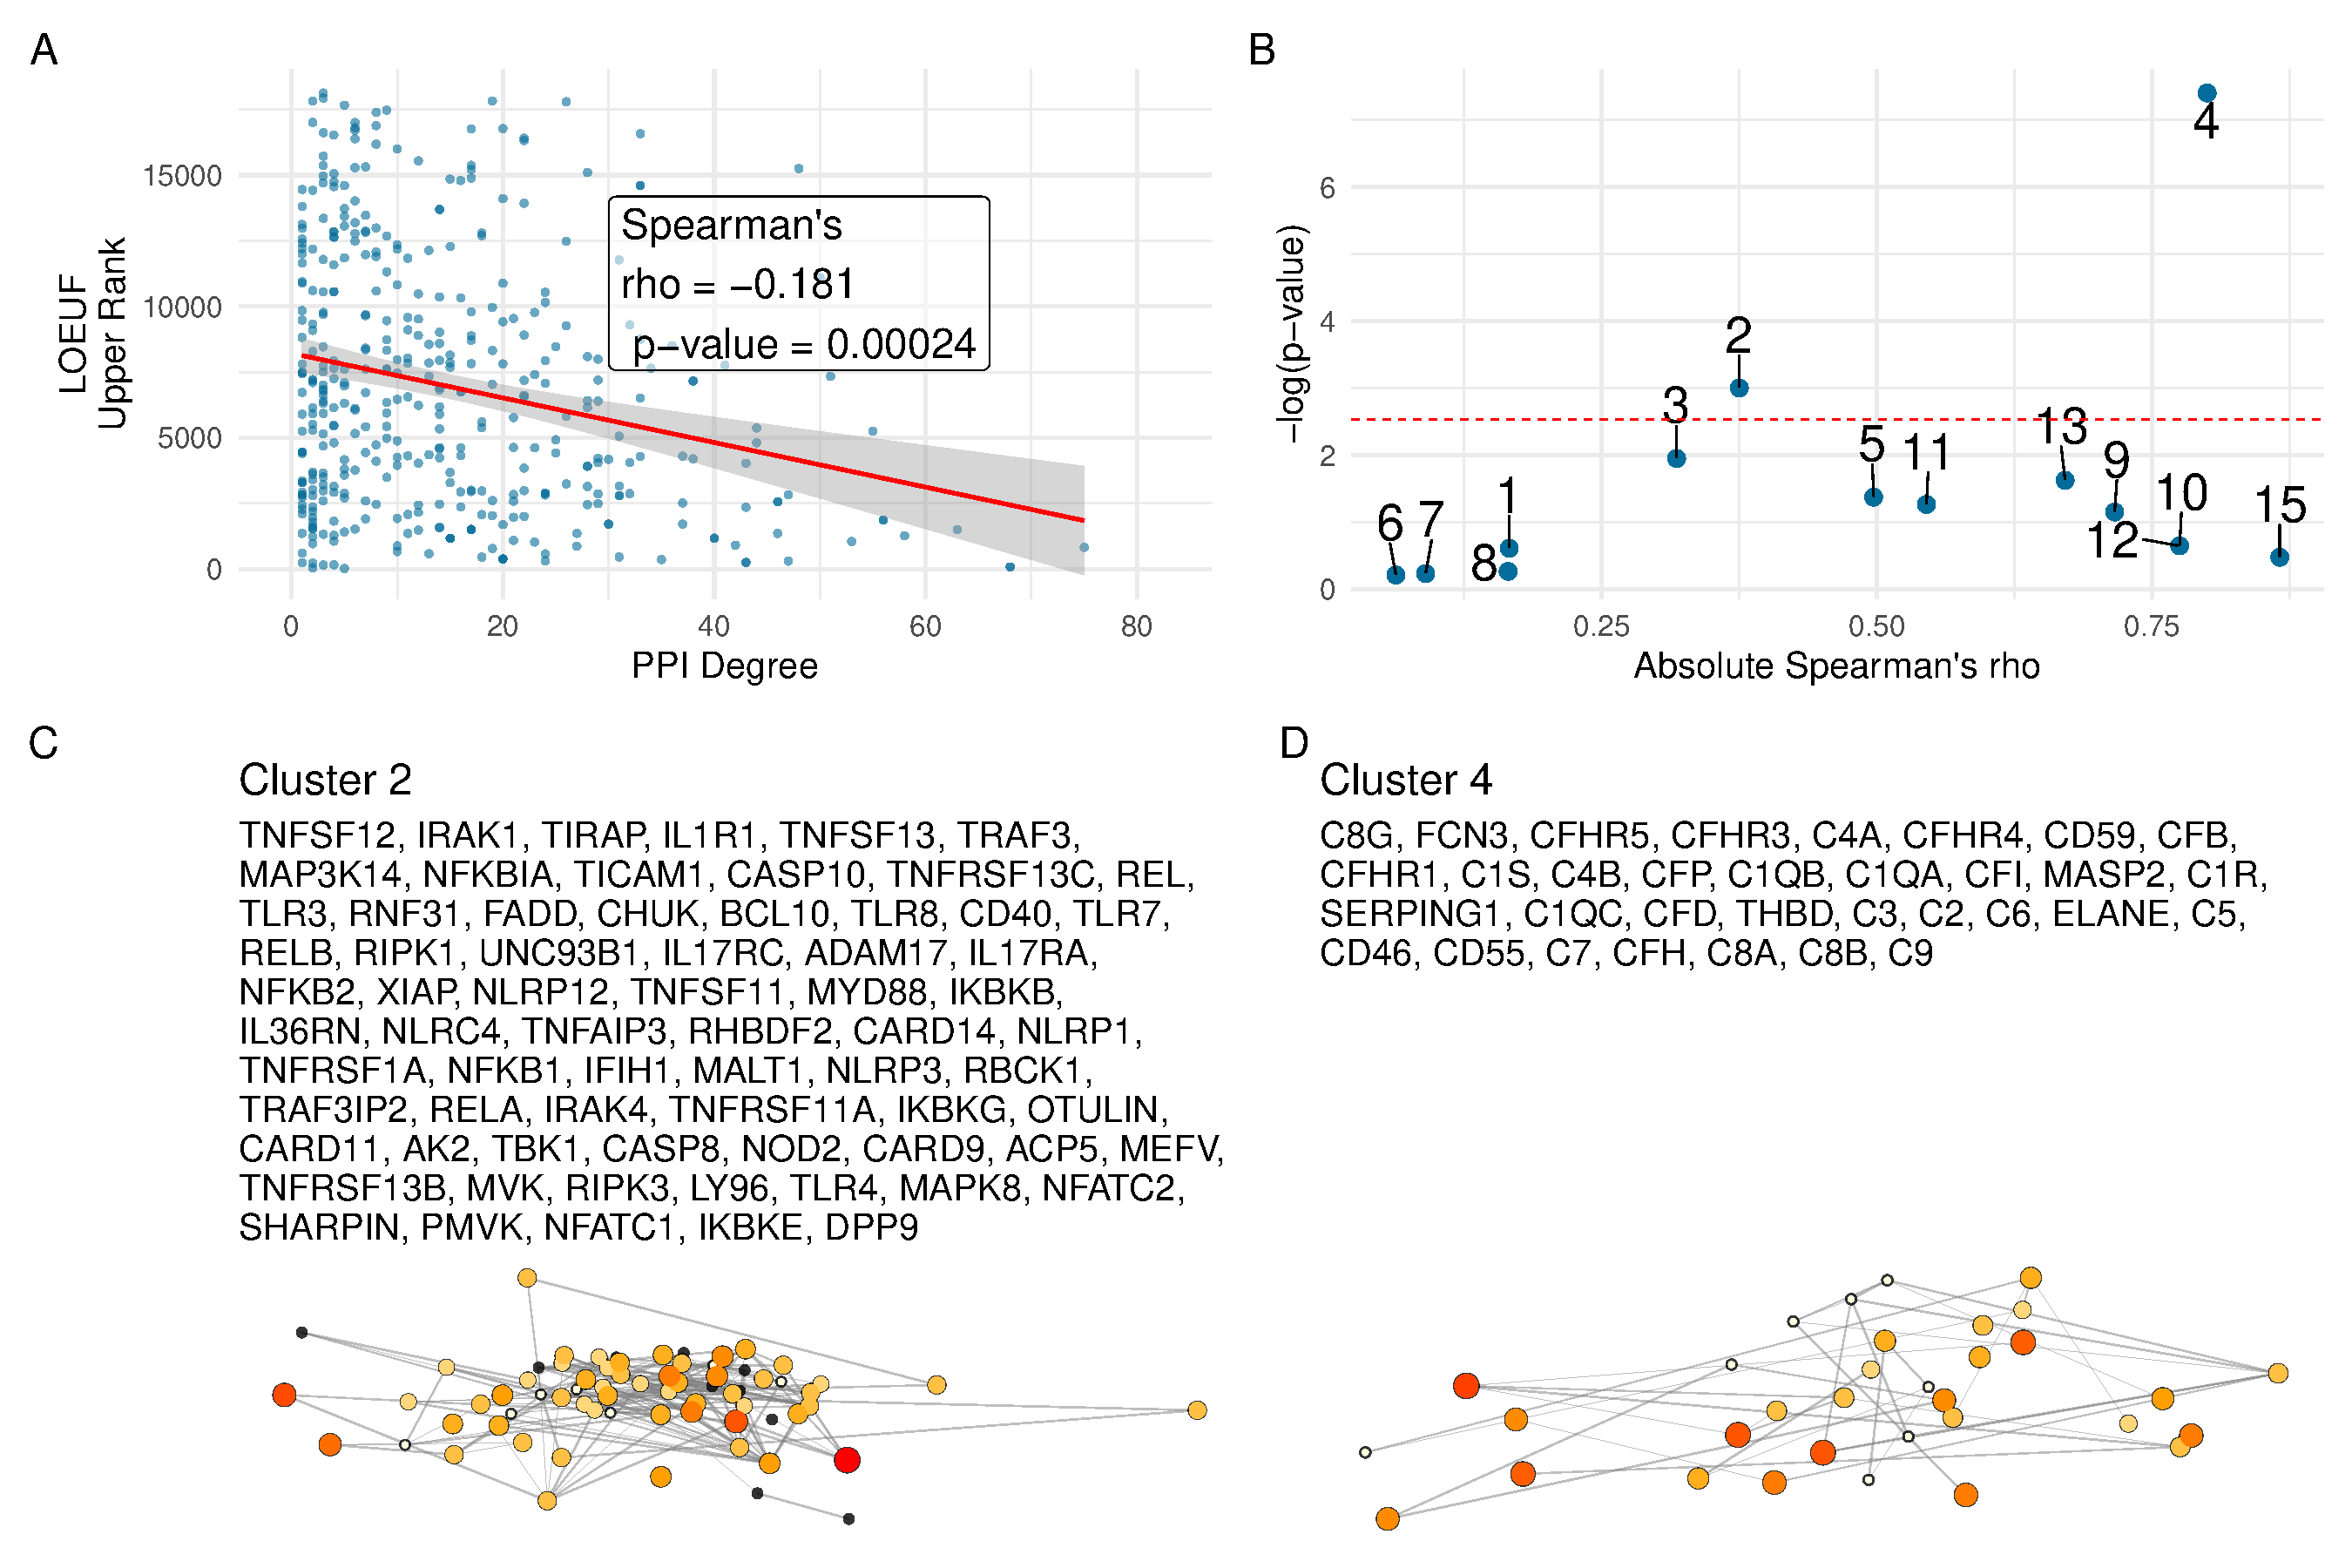
\includegraphics[width=0.99\textwidth]{../images/untangleR_ppi_network_p_cor_spear_rho_sig_clust_patch3.pdf}
  \caption{
    \textbf{Correlation between PPI degree and LOEUF upper rank.} 
    \textbf{(A)} Ananlysis across all genes revealed a weak, significant negative correlation (ρ = –0.181, p = 0.00024) between PPI degree and LOEUF upper rank. \textbf{(B)} The cluster-wise analysis showed that clusters 2 (ρ = –0.375, p = 0.000994) and 4 (ρ = –0.800, p < 0.000001) exhibit moderate to strong correlations, while other clusters display weak or non-significant relationships. \textbf{(C) and (D)} Shows the new network plots for the significantly enriched clusters based on gnomAD constraint metrics.
  }
  \label{fig:p_cor_spear_rho_sig_clust_patch3}
\end{figure}

% \subsubsection{Network Analysis of Enriched Significant Clusters Based on gnomAD Constraint}
\textbf{Figure \ref{fig:p_cor_spear_rho_sig_clust_patch3} (C, D)} shows the re-plotted PPI networks for clusters with significant correlations between PPI degree and LOEUF upper rank. In these networks, node size is scaled by a normalised variant score, while node colour reflects the variant score according to a predefined palette.

\FloatBarrier
%
%\subsubsection{Integration of Variant Probabilities into IEI Genetics Data} 
%Provides a summary of how variant probabilities are incorporated into the broader IEI genetics framework (Figure 6).
%
%The underlying data containing the probabilities of observing a variant classification for a human with the given phenotype were then reintegrated back into our publicly accessible tool.
%We provide the raw data in the Zenodo repository. 
%Figure \ref{fig:var_risk_est_iei_genetics} displays the interface used to summarise this condensed data.
%
%
%\begin{figure}[ht]
%  \centering
%  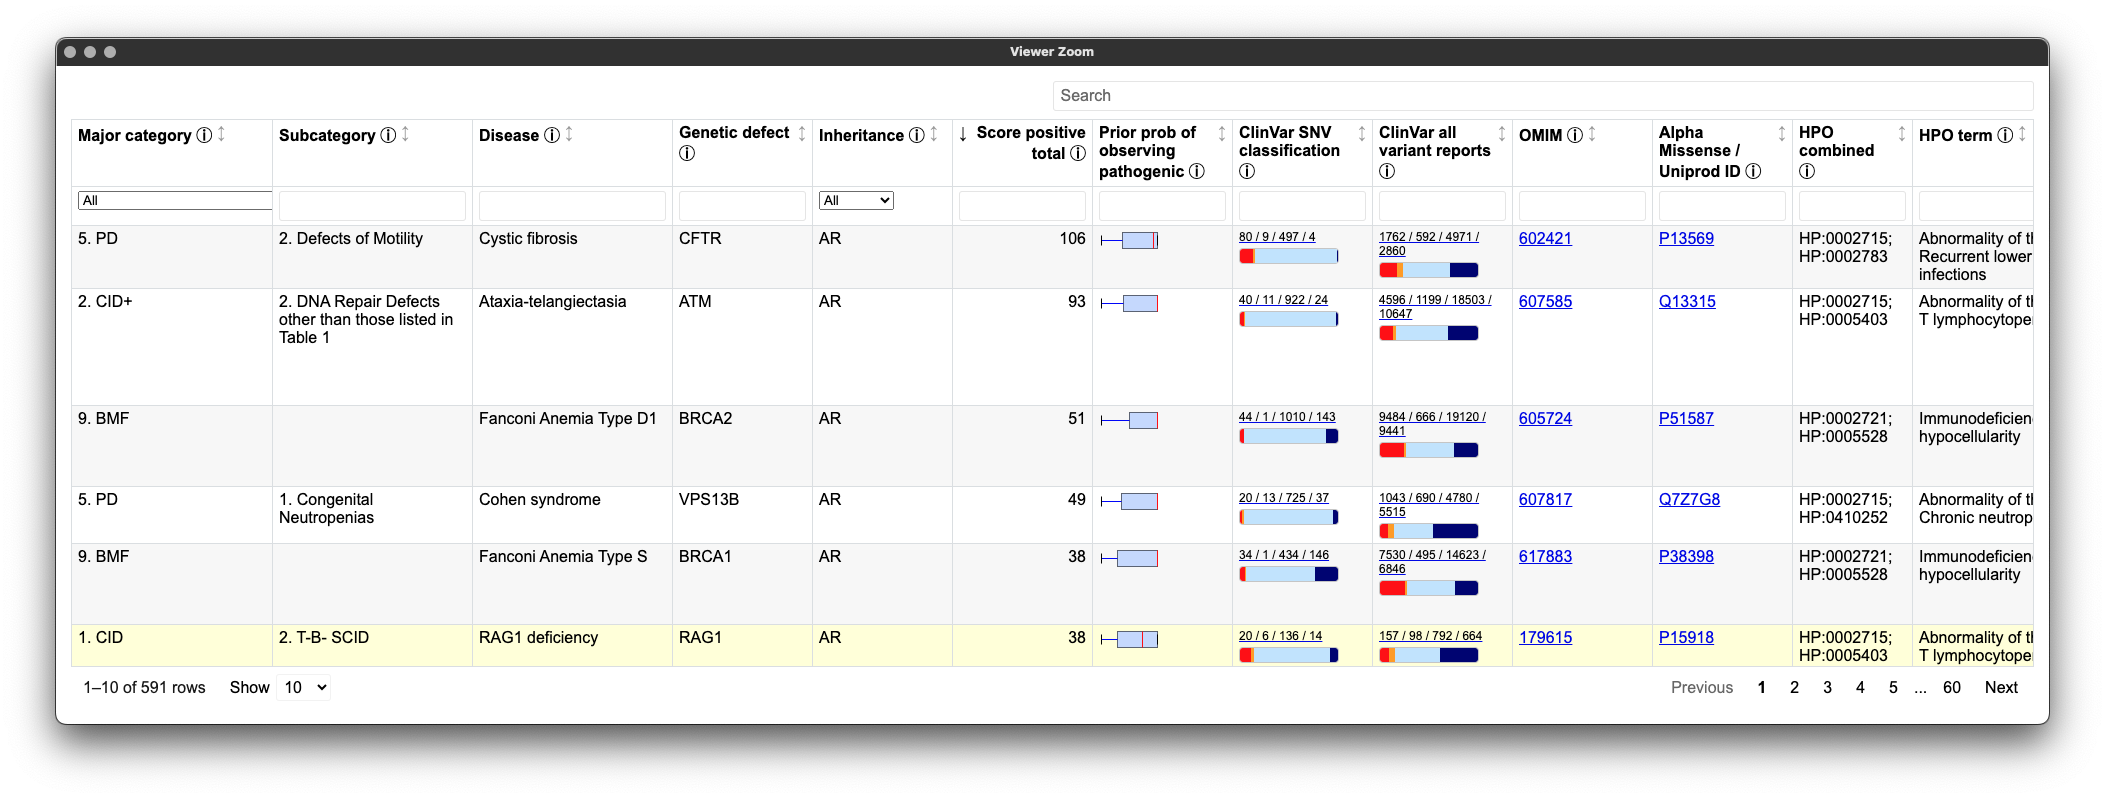
\includegraphics[width=0.99\textwidth]{../images/var_risk_est_iei_genetics.png}
%  \caption{Variant probabilities integrated back into our IEI genetics table and PanelAppRex.}
%  \label{fig:var_risk_est_iei_genetics}
%\end{figure}
%
%
%We pre‐calculate summary statistics server‐side to reduce browser rendering load when visualising large genomic datasets. Score mapping converts clinical significance terms into numeric values, distilling complex data into key metrics (e.g. counts of pathogenic classifications) while filtering incidental benign variants, which nonetheless inform prior false‐positive odds. We summarise both pathogenic and benign data and integrate visual summaries (stacked bar charts, classification counts) into a responsive layout. For the “prior probability of observing pathogenic” variants, we compute key quantiles (min, Q1, median, Q3, max) of the probability distribution for each gene and render a compact sparkline box plot per table row. Finally, dynamic URL generation (using sprintf and htmltools tags) links table entries to source databases (e.g. ClinVar, OMIM, AlphaFold), ensuring immediate access to comprehensive external information.
%
%
%

\subsubsection{Integration of Variant Probabilities into IEI Genetics Data}
We integrated the computed prior probabilities for observing variants in all known genes associated with a given phenotype, across autosomal dominant, autosomal recessive, and X-linked modes of inheritance, into our IEI genetics framework. These calculations, derived from gene panels in PanelAppRex, have yielded novel insights for the IEI disease panel. The final result comprised of machine- and human-readable datasets, including the table of variant classifications and priors available via a Zenodo repository, and a user-friendly web interface that incorporates these new metrics.

\textbf{Figure \ref{fig:var_risk_est_iei_genetics}} shows the interface summarising integrated variant data. Server-side pre-calculation of summary statistics minimises browser load, while clinical significance is converted to numerical metrics. Key quantiles (min, Q1, median, Q3, max) for each gene are rendered as sparkline box plots, and dynamic URLs link table entries to external databases (e.g. ClinVar, OMIM, AlphaFold).


\begin{figure}[ht]
  \centering
  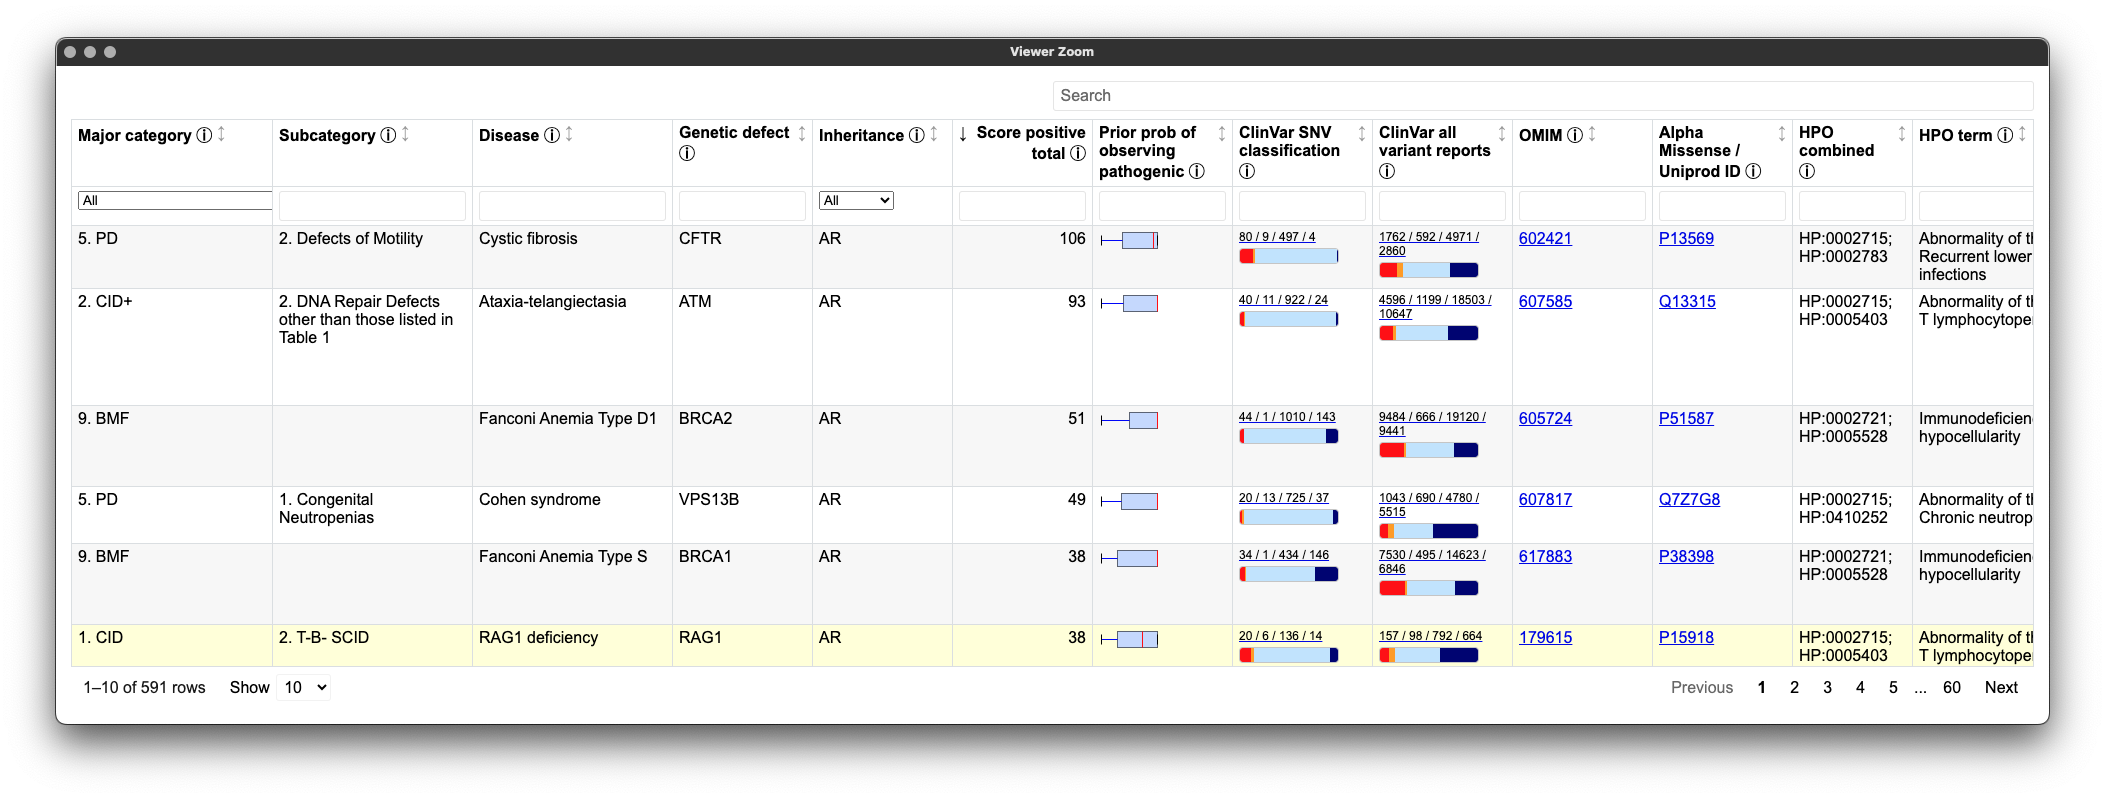
\includegraphics[width=0.99\textwidth]{../images/var_risk_est_iei_genetics.png}
  \caption{
    \textbf{Integration of variant probabilities into the IEI genetics framework.}
    The interface summarises the condensed variant data, with pre-calculated summary statistics and dynamic links to external databases. This integration enables immediate access to detailed variant classifications and prior probabilities for each gene.
  }
  \label{fig:var_risk_est_iei_genetics}
\end{figure}




\FloatBarrier
%\section{Discussion}
%
%In this study, we focused on quantifying the probability of disease observation by integrating large-scale genomic annotation with classical genetic principles. Our analysis of 54,814 ClinVar variant classifications across 557 genes in PanelAppRex’s panel (ID 398) for primary immunodeficiency or monogenic inflammatory bowel disease exemplifies how genome-wide assessments of gene–disease combinations can be performed \cite{lawless_panelapprex_2025}. 
%By processing curated data sources, including population allele frequencies from gnomAD
%\cite{karczewski2020mutational}, variant classifications from ClinVar \cite{landrum_clinvar_2018}, and functional annotations as summarised in sources like dbNSFP, and by rigorously applying HWE-related calculations, we derived robust estimates of the likelihood of observing disease-associated variants. 
%Our method accounts for the complexities of different inheritance modes; for instance, while autosomal dominant (AD) and X-linked (XL) disorders require only a single pathogenic allele, autosomal recessive (AR) conditions necessitate the consideration of both homozygous and compound heterozygous states.
%
%The classical HWE-based estimates obtained here serve as robust priors for Bayesian models of variant and disease risk estimation, an approach that is frequently underutilised in clinical and statistical genetics. Our framework not only refines risk calculations by incorporating inheritance complexities but also enriches clinicians’ understanding of expected variant occurrences in a patient, thereby improving diagnostic precision. Moreover, the integration of established variant interpretation guidelines such as those provided by the ACMG \citep{richards2015standards} and complementary frameworks \citep{tavtigian2020fitting,li2017intervar}, alongside standardized quality control protocols \citep{pedersen2021effective,anderson2010data}, reinforces the clinical relevance of our estimates.
%
%Our study further demonstrates that statistical methods for aggregating variant effects (e.g., ACAT and SKAT \citep{liu2019acat,li2020dynamic,wu2011rare,lee2012optimal}) and multi-block data fusion techniques for integrating diverse omics layers \citep{kong2018nature,howe2021within} can be effectively supplemented by our observation probability framework. In addition, standardized reporting for qualifying variant sets, such as ACMG Secondary Findings v3.2 \citep{miller2023acmg}, provides further context for the integration of these probabilities into clinical decision-making.
%
%We acknowledge that our current approach is limited to single nucleotide variants (SNVs) and does not account for  other complexities of genetic disease,
%including complex variants, de novo events, hypomorphic phenotypes,
%overdominance, penetrance, tissue-specific transcription, pleiotropy, etc.
%\cite{zschocke_mendelian_2023}.
%
%Future work will incorporate additional variant types and models to further refine these probability estimates. By continuously updating classical estimates with emerging data and prior knowledge, we hope to enhance the precision of genetic diagnostics and ultimately improve patient care.
%

\section{Discussion}

Our study presents, to our knowledge, the first comprehensive framework for calculating prior probabilities of observing disease-associated variants across all modes of inheritance for any gene–disease combination. By integrating large-scale genomic annotations, including population allele frequencies from gnomAD \cite{karczewski2020mutational}, variant classifications from ClinVar \cite{landrum_clinvar_2018}, and testing against functional annotations from resources such as dbNSFP, with classical Hardy-Weinberg-based calculations, we derived robust estimates for 54,814 ClinVar variant classifications across 557 genes implicated in primary immunodeficiency and monogenic inflammatory bowel disease \cite{lawless_panelapprex_2025}. 

Our genome-wide approach accommodates the distinct inheritance patterns of autosomal dominant (AD), autosomal recessive (AR), and X-linked (XL) disorders. Whereas AD and XL conditions require only a single pathogenic allele, AR disorders necessitate the consideration of both homozygous and compound heterozygous states. These classical HWE-based estimates provide an informative baseline for predicting variant occurrence and serve as robust priors for Bayesian models of variant and disease risk estimation. This is an approach that has been underutilised in clinical and statistical genetics. As such, our framework refines risk calculations by incorporating inheritance complexities and enhances clinicians’ understanding of expected variant occurrences, thereby improving diagnostic precision.

Moreover, our method complements existing statistical approaches for aggregating variant effects (e.g., ACAT and SKAT \cite{liu2019acat,li2020dynamic,wu2011rare,lee2012optimal}) and multi-omics integration techniques \cite{kong2018nature,howe2021within}, while remaining consistent with established variant interpretation guidelines from the ACMG \cite{richards2015standards} and complementary frameworks \cite{tavtigian2020fitting,li2017intervar}, as well as quality control protocols \cite{pedersen2021effective,anderson2010data}. Standardised reporting for qualifying variant sets, such as ACMG Secondary Findings v3.2 \cite{miller2023acmg}, further contextualises the integration of these probabilities into clinical decision-making.

We acknowledge that our current approach is limited to single nucleotide variants (SNVs) and does not account for other complexities of genetic disease, including complex variants, de novo events, hypomorphic phenotypes, overdominance, penetrance, tissue-specific transcription, and pleiotropy \cite{zschocke_mendelian_2023}. Future work will incorporate additional variant types and models to further refine these probability estimates. By continuously updating classical estimates with emerging data and prior knowledge, we aim to enhance the precision of genetic diagnostics and ultimately improve patient care.

\section{Conclusion}
Our work generates prior probabilities for observing any variant classification in IEI genetic disease, providing a quantitative resource to enhance Bayesian variant interpretation and clinical decision-making.

\section*{Acknowledgements}
\noindent
We acknowledge Genomics England for providing public access to the PanelApp data.
The use of data from Genomics England panelapp was licensed under the Apache License 2.0.
The use of data from UniProt was licensed under Creative Commons Attribution 4.0 International (CC BY 4.0).
ClinVar asks its users who distribute or copy data to provide attribution to them as a data source in publications and websites \cite{landrum_clinvar_2018}.
dbNSFP version 4.4a is licensed under the Creative Commons Attribution-NonCommercial-NoDerivatives 4.0 International (CC BY-NC-ND 4.0); while we cite this dataset as used our research publication, it is not used for the final version which instead used ClinVar and gnomAD directly.
GnomAD is licensed under  Creative Commons  Zero Public Domain Dedication (CC0 1.0 Universal).
GnomAD request that usages cites the gnomAD flagship paper \cite{karczewski2020mutational}
and any online resources that include the data set provide a link to the browser, and note that tool includes data from the gnomAD v4.1 release.

\section*{Competing interest}
\noindent
We declare no competing interest. 

\newpage
\bibliographystyle{unsrtnat}
\bibliography{references}

\clearpage
%\\\\\\\\\\\\\\\\\\\\\\\\\\\\
\beginsupplement
\section{Supplemental} \label{Supplemental_text}

\begin{figure}[ht]
  \centering
  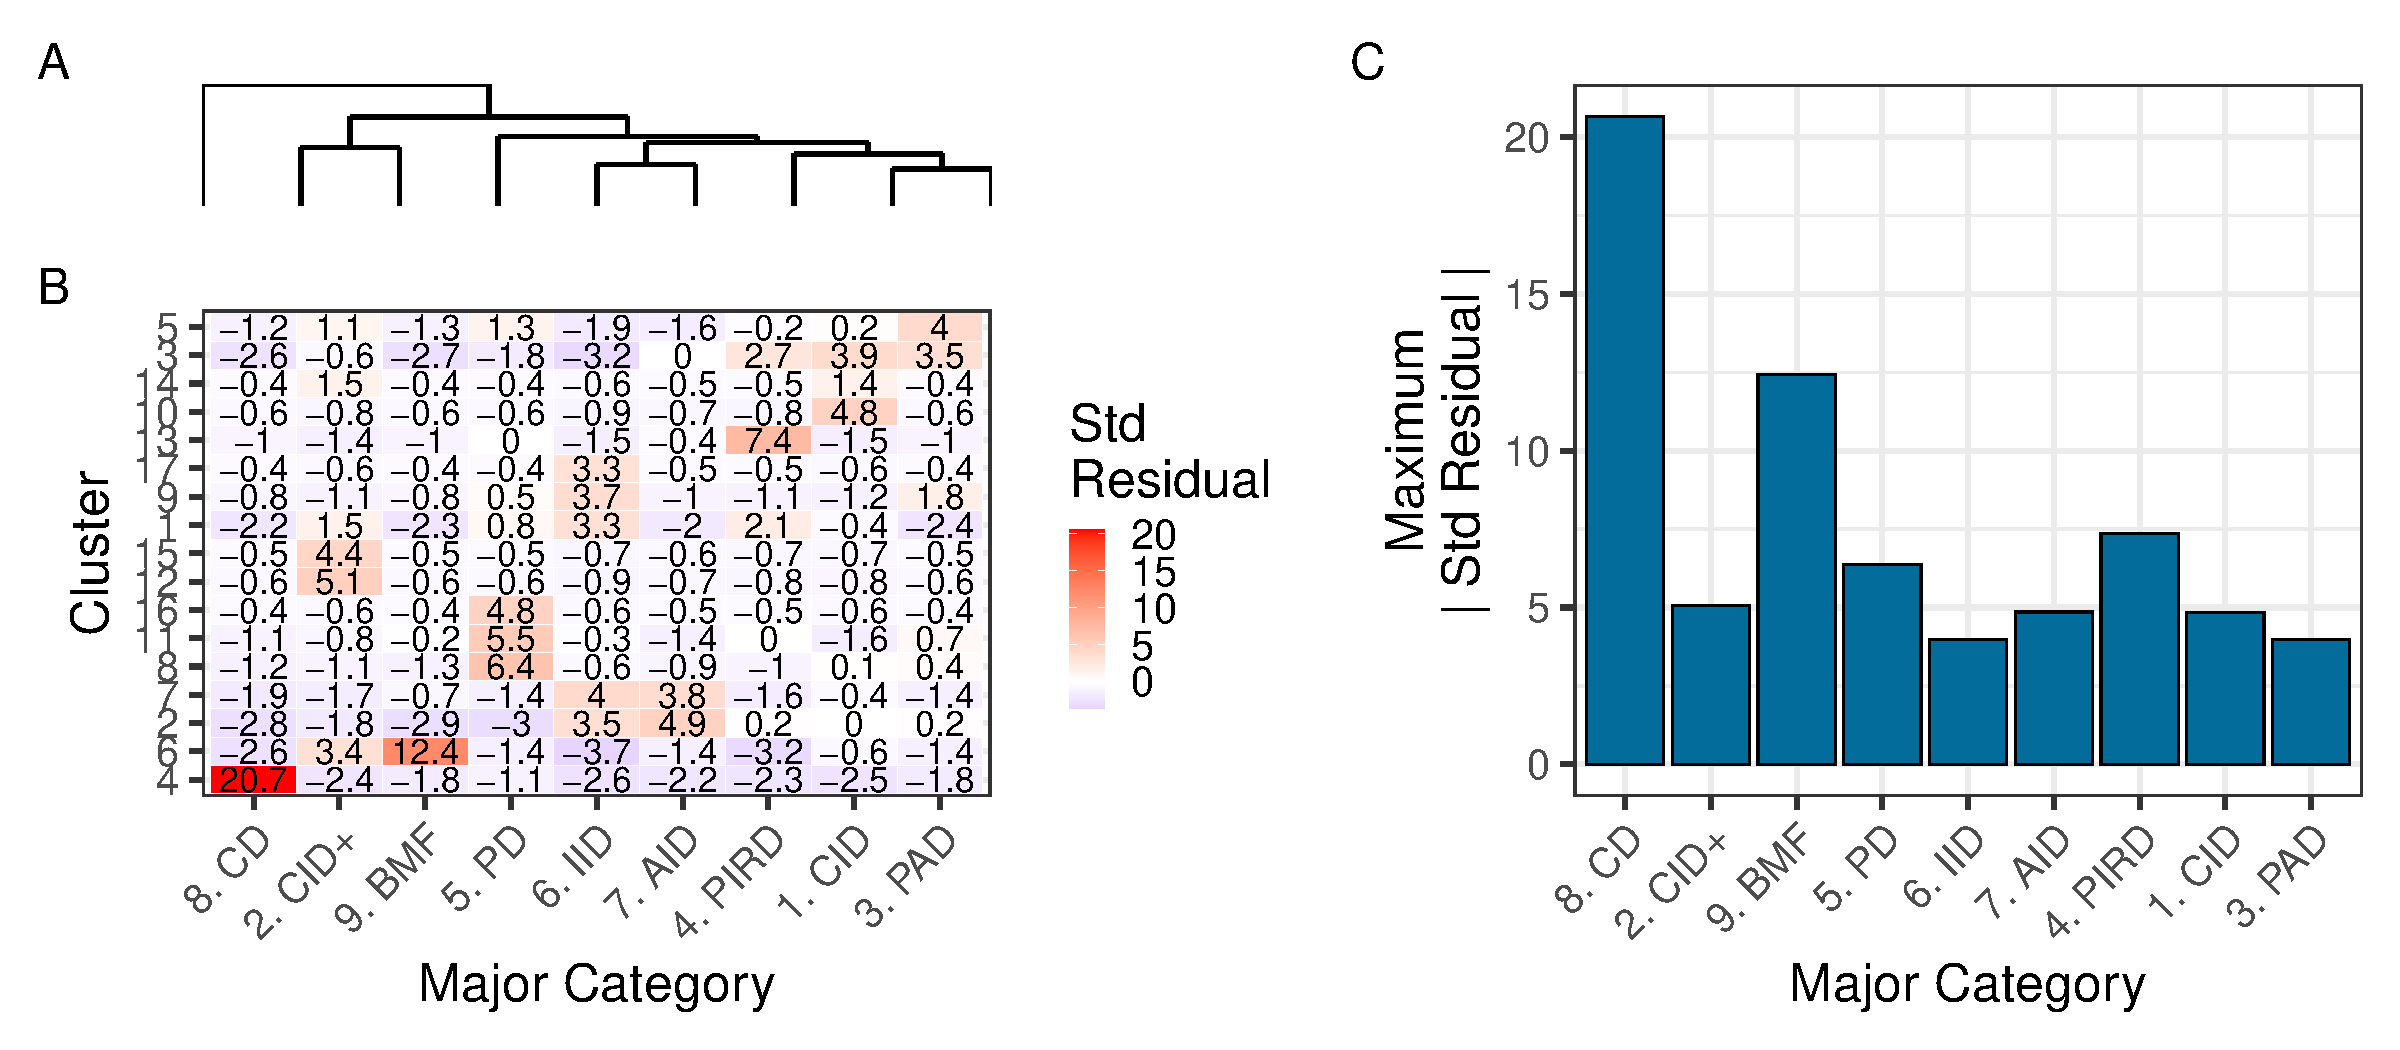
\includegraphics[width=0.99\textwidth]{../images/untangleR_ppi_network_patch2_cator.pdf}
  \caption{
    Hierarchical clustering of enrichment scores.
    The heatmap displays standardised residuals for major disease categories (x-axis) across network clusters (y-axis). A dendrogram groups similar disease categories, and the bar plot shows the maximum absolute residual per category. Cet 8.CD and 9, BMF show the highest values, indicating significant enrichment or depletion (residuals > |2|). Definitions in \textbf{Box \ref{box:definitions}}.
  }
  \label{fig:patch2}
\end{figure}

\begin{figure}[ht]
  \centering
  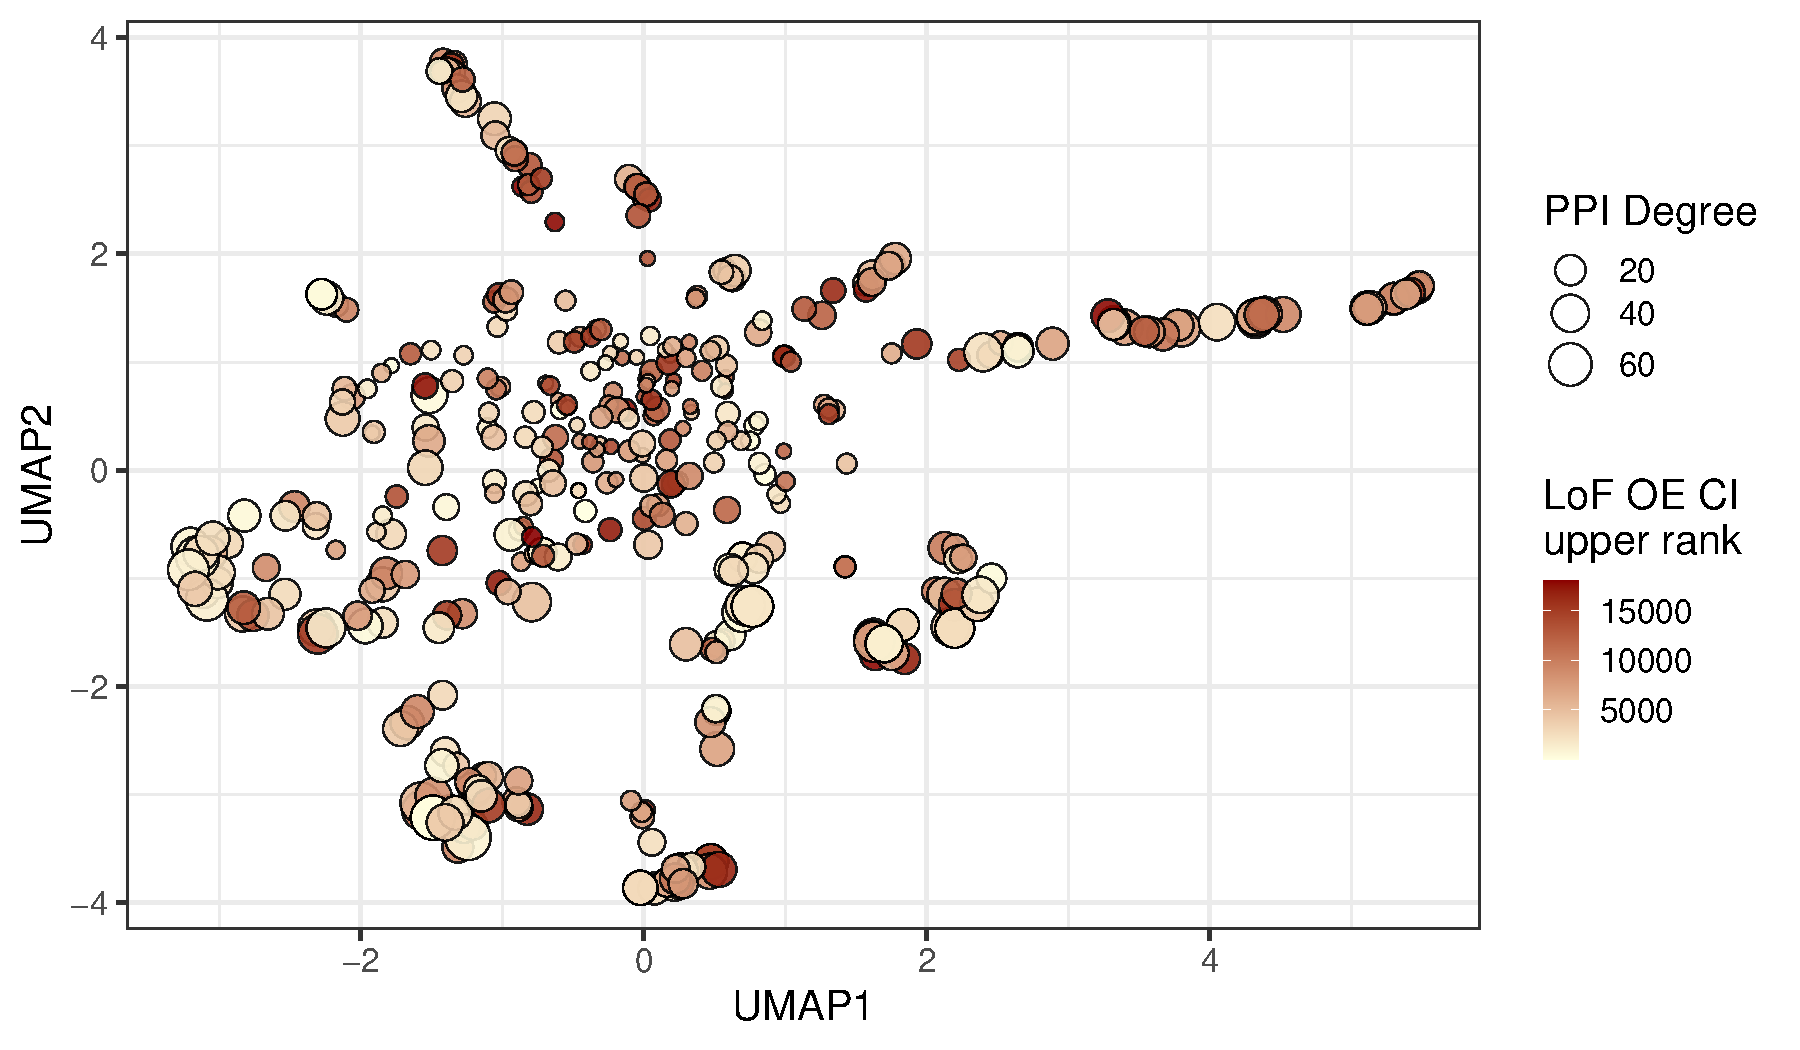
\includegraphics[width=0.99\textwidth]{../images/untangleR_ppi_network_p_umap_const.pdf}
  \caption{
   Supplementary analysis of PPI degree versus LOEUF upper rank with UMAP embedding of the PPI network.
    The relationship between PPI degree (size) and LOEUF upper rank (color) across gene clusters. No clear patterns are evident.
  }
  \label{fig:p_umap_const}
\end{figure}


\end{document}
